%%%%%%%%%%%%%%%%%%%%%%%%%%%%%%%%%%%%%%%%%%%%%%%%%%%%%%%%%%%%%%%%%%%%%%%%%%%%%%%
% Delovni osnutek diplomske naloge - bachelor-thesis-book
% Pred oddajo nastavite \thesisdraftfalse in odstranite vsa navodila TODO.
%%%%%%%%%%%%%%%%%%%%%%%%%%%%%%%%%%%%%%%%%%%%%%%%%%%%%%%%%%%%%%%%%%%%%%%%%%%%%%%

% !BIB program = biber
\DocumentMetadata{
  pdfstandard = A-4,
  pdfversion  = 2.0,
  lang        = sl-SI,
  colorprofiles = {sRGB_v4_ICC_preference.icc}
}

\documentclass[a4paper,12pt,openright]{book}

%%%%%%%%%%%%%%%%%%%%%%%%%%%%%%%%%%%%%%%%
% PODATKI O DIPLOMI
%%%%%%%%%%%%%%%%%%%%%%%%%%%%%%%%%%%%%%%%

\newcommand{\tauthor}{Aleks Muhič}
\newcommand{\temail}{am8139@student.uni-lj.si}
\newcommand{\tmentor}{viš.~pred.~dr.~Robert Rozman}

\newcommand{\tstopnja}%
{VISOKOŠOLSKI STROKOVNI ŠTUDIJSKI PROGRAM\\ PRVE STOPNJE}

\newcommand{\tinst}%
{Fakulteta za računalništvo in informatiko}

\newcommand{\tvrsta}{Diplomska naloga na visokošolskem programu prve stopnje}

% Pred oddajo dobesedno prepišite opis, ki ga mentor vnese v StudIS.
\newcommand{\tdescription}
{Cilj diplomskega dela je razviti in ovrednotiti vgrajeni sistem za sprotno
zaznavanje nevarnih zvočnih dogodkov na razvojni plošči STM32N6570-DK.
Sistem je zasnovan kot prototip vidnega opozarjanja za gluhe in naglušne osebe,
pri čemer se zvok obdeluje lokalno brez dostopa do računalniškega oblaka in
brez trajnega shranjevanja surovih zvočnih posnetkov.
Kandidat bo prilagodil kvantizirani model na osnovi arhitekture YAMNet za
izvajanje na mikrokrmilniku STM32N6 z nevronskim pospeševalnikom Neural-ART ter
povezal zajem zvoka, predobdelavo, sklepanje in prikaz rezultatov. Sistem bo
ovrednotil z nadzorovanim preskusom na fizični napravi ter analiziral pravilnost
zaznavanja, lažne alarme, čas izvajanja in porabo pomnilnika.}

\newcommand{\tdescriptionEn}
{The aim of the thesis is to develop and evaluate an embedded system for
real-time hazardous sound event detection on the STM32N6570-DK development
board. The system is designed as a visual-alert prototype for deaf and hard of
hearing users, with local audio processing, no cloud access, and no persistent
storage of raw audio recordings. The candidate will adapt a quantized model based on the YAMNet
architecture for execution on an STM32N6 microcontroller with the Neural-ART
accelerator and integrate audio acquisition, preprocessing, inference, and
result presentation. The system will be evaluated through a controlled test on
the physical device, including detection performance, false alerts, execution
time, and memory usage.}

\newcommand{\ttitle}
{Razvoj in vrednotenje sistema za zaznavanje nevarnih zvočnih dogodkov na
mikrokrmilniku STM32N6 z uporabo nevronskega pospeševalnika}

\newcommand{\ttitleEn}
{Development and Evaluation of a Hazardous Sound Event Detection System on an
STM32N6 Microcontroller with a Neural Accelerator}

\newcommand{\tkeywords}
{vgrajeni sistemi, zaznavanje zvočnih dogodkov, STM32N6, nevronski
pospeševalnik, robna umetna inteligenca, zasebnost}

\newcommand{\tkeywordsEn}
{embedded systems, sound event detection, STM32N6, neural accelerator, edge AI,
privacy}

% Delovni mesti; pred oddajo besedilo dopolnite ali izpustite.
\newcommand{\tzahvala}
{[Dopolnite zahvalo ali jo pred oddajo odstranite.]}

\newcommand{\tposvetilo}{}

\input{podporno/preambula.tex}

% Vidna navodila so namenjena pisanju in niso del končnega besedila.
\newif\ifthesisdraft
\thesisdrafttrue
\newcommand{\draftnote}[1]{%
  \ifthesisdraft
    \par\medskip
    \noindent\fbox{\parbox{0.92\textwidth}{\small
      \textbf{Navodilo za pisanje:} #1}}
    \par\medskip
  \fi
}

\begin{document}

\newcommand{\tpovzetek}
{V diplomskem delu je predstavljen samostojen vgrajeni sistem, ki izbrane
nevarne zvočne dogodke pretvori v vidno opozorilo. Namenjen je kot raziskovalni
prototip pomoči gluhim in naglušnim osebam. Celotna obdelava poteka lokalno na
razvojni plošči STM32N6570-DK, zato sistem ne potrebuje dostopa do
računalniškega oblaka, običajna različica programa pa ne shranjuje surovih
zvočnih posnetkov. Zvok zajema vgrajeni mikrofon, predobdelava izračuna
logaritemski melov spektrogram, kvantizirani model YAMNet-1024 pa se izvaja z
nevronskim pospeševalnikom Neural-ART. Ciljni model razpoznava pasji lajež,
razbitje stekla, strel, sireno, govor in druge zvoke. Stabilnost prikaza
zagotavljajo pragovi po razredih in časovno filtriranje. V neodvisnem fizičnem
preizkusu je sistem pričakovani razred vsaj enkrat potrdil v 57 od 60 poskusov,
pri štirih nevarnostnih razredih pa v 39 od 40 poskusov. Obdelava enega bloka
je trajala 10,81 milisekunde. Rezultati potrjujejo izvedljivost lokalnega
razpoznavanja v realnem času, hkrati pa pokažejo potrebo po boljšem zavračanju
nekaterih kratkih običajnih zvokov.}

\newcommand{\tabstract}
{This thesis presents a self-contained embedded system that converts selected
hazardous sound events into visual alerts. It is intended as a research
prototype to assist deaf and hard of hearing users. All processing runs locally
on an STM32N6570-DK development board, so the system requires no cloud access,
and the normal firmware does not retain raw audio recordings. Audio is captured
by the onboard microphone, preprocessing produces a log-mel spectrogram, and a
quantized YAMNet-1024 model runs on the Neural-ART accelerator. The targeted
model recognizes dog barks, breaking glass, gunshots, sirens, speech, and other
sounds. Per-class thresholds and temporal filtering stabilize the displayed
decision. In an independent physical evaluation, the system confirmed the
expected class at least once in 57 of 60 trials and in 39 of 40 trials covering
the four hazardous classes. Processing one input block took 10.81 milliseconds.
The results demonstrate the feasibility of local real-time recognition while
also showing that rejection of some short everyday sounds requires further
improvement.}

\input{podporno/naslovnestrani.tex}

\mainmatter
\setcounter{page}{1}
\pagestyle{fancy}

\chapter{Uvod}
\label{ch:uvod}

Poglavje predstavi motivacijo za lokalno zaznavanje nevarnih
zvočnih dogodkov. Nato opredeli cilje in raziskovalna vprašanja, glavne
prispevke ter zgradbo preostalega dela.

\section{Motivacija in opredelitev problema}

Zvočni dogodki, kot so sirena, razbitje stekla, strel ali pasji
lajež, lahko človeka opozorijo na nevarnost, še preden jo opazi. Gluhe in
naglušne osebe zvočnega opozorila ne morejo vedno zaznati. Namen rešitve je zato
zvok iz okolice sproti pretvoriti v vidno informacijo na zaslonu. Cilj dela ni
razviti medicinskega ali varnostno certificiranega pripomočka, temveč preveriti,
ali je mogoče celotno pot od mikrofona do uporabniškega opozorila izvesti na
računsko in pomnilniško omejeni napravi.

Običajen pristop bi lahko zvočne posnetke pošiljal v oddaljeno računalniško
okolje, kjer bi jih obdelal večji model. Takšna rešitev je odvisna od omrežne
povezave, hkrati pa neprekinjen prenos zvoka iz domačega okolja odpira vprašanja
zasebnosti. V tej nalogi se vsi koraki izvajajo lokalno na razvojni plošči, brez
shranjevanja zvočnih podatkov. Takšna zasnova zmanjšuje izpostavljenost zasebnih
podatkov in omogoča delovanje brez dostopa do interneta.

Lokalna izvedba prinese strožje tehnične omejitve. Mikrokrmilnik mora
neprekinjeno zajemati zvok, izračunati strnjeni spektrogram, izvesti
nevronsko mrežo, filtrirati nestabilne napovedi in osveževati zaslon. Vse to
mora opraviti z omejenim pomnilnikom in dovolj hitro, da med računanjem ne
izgubi novih vzorcev. Poleg hitrosti je pomembno tudi zavračanje običajnih
zvokov. Naloga zato obravnava tako izvajanje modela z nevronskim
pospeševalnikom kot tudi merjenje pravilnih zaznav in lažnih alarmov na napravi.

\section{Cilji in raziskovalna vprašanja}

Glavni cilj je razviti delujoč vgrajeni sistem na razvojni plošči
STM32N6570-DK, ki z vgrajenim mikrofonom zaznava izbrane nevarne zvočne
dogodke in rezultat brez omrežne povezave prikaže na zaslonu. Sistem razlikuje
med naslednjimi zvočnimi razredi:

\begin{itemize}
\item pasji lajež,
\item razbitje stekla,
\item strel,
\item sirena,
\item govor in
\item ostalo.
\end{itemize}

Poleg zvočnih razredov lahko sistem prikaže še dve stanji:

\begin{itemize}
\item negotovo napoved in
\item čakanje na dogodek.
\end{itemize}

Dodatni cilj je pripraviti ponovljiv postopek vrednotenja, s katerim je mogoče
točno različico modela in programa povezati z izmerjenimi rezultati.

V nalogi odgovarjamo na naslednja raziskovalna vprašanja:

\begin{enumerate}
  \item Ali je mogoče kvantizirani model za zaznavanje zvočnih dogodkov
        izvajati v realnem času na mikrokrmilniku STM32N6 z uporabo
        nevronskega pospeševalnika Neural-ART?
  \item Kakšen delež potrjenih pravilnih zaznav in lažnih nevarnostnih alarmov
        doseže končni sistem pri nadzorovanem predvajanju zvokov na fizični
        napravi?
  \item Kako se posamezni zvočni razredi razlikujejo po uspešnosti klasifikacije in kateri
        dejavniki omejujejo delovanje sistema?
\end{enumerate}

Prvo vprašanje obravnava čas izvajanja in porabo pomnilnika, drugo uspešnost
zaznavanja in lažne alarme pri preizkusu na fizični napravi, tretje pa razlike
v uspešnosti klasifikacije med razredi in omejitve sistema.

Model in odločitvena pravila so bili izbrani z učnimi in razvojnimi podatki.
Končni preizkus je uporabil 60 novih zvočnih virov, ki pri učenju ali izbiri
pragov niso bili uporabljeni.

\section{Prispevki diplomskega dela}

Glavni prispevki dela so:

\begin{itemize}
  \item povezava neprekinjenega zajema z vgrajenega mikrofona, digitalne
        predobdelave, modela YAMNet-1024 in nevronskega pospeševalnika v
        samostojno delujočo aplikacijo;
  \item priprava ciljnega učnega postopka z izrezovanjem kratkotrajnih dogodkov,
        povečanjem podatkov ter dodatnima razredoma govor in ostalo;
  \item izvedba časovnega filtra s pragovi po razredih ter uporabniškega
        vmesnika, ki prikazuje trenutno in nedavne napovedi;
  \item lokalna zasnova brez pošiljanja zvoka v računalniški oblak in brez
        trajnega shranjevanja surovih zvočnih vzorcev v običajnem delovanju;
  \item sledljiv realni preizkus s 60 novimi, slušno pregledanimi zvočnimi
        dražljaji, shranjenimi dnevniki, kontrolnimi vsotami in ponovljivo
        analizo rezultatov.
\end{itemize}

Prednaučeni model YAMNet-1024 ni bil razvit v okviru te naloge. V nalogi smo
naučili novo izhodno plast, ki izhod modela razvrsti v izbrane zvočne razrede.
Pripravili smo tudi podatke, model prilagodili za izvajanje na mikrokrmilniku,
razvili pravila za prikaz rezultatov in ovrednotili delovanje celotnega sistema.

\section{Opis vsebine dela}

V poglavju \ref{ch:teorija} so predstavljene osnove digitalnega
zvoka, strnjenega spektrograma, nevronskih mrež in kvantizacije. Poglavje
\ref{ch:zasnova} opredeli zahteve, strojno platformo ter tok podatkov, poglavje
\ref{ch:implementacija} pa podrobno opiše zajem zvoka, predobdelavo, pripravo
modela, izvajanje na pospeševalniku in uporabniški vmesnik. Metodologija
razvojnih in končnih preskusov je podana v poglavju \ref{ch:metodologija},
izmerjeni rezultati v poglavju \ref{ch:rezultati}, odgovori na raziskovalna
vprašanja, omejitve projekta in sklepne ugotovitve pa v poglavju
\ref{ch:razprava-sklep}.

\chapter{Teoretične osnove in sorodna dela}
\label{ch:teorija}

Poglavje predstavi osnove, potrebne za razumevanje celotne poti od
zvoka v prostoru do prikazane odločitve. Najprej je opisan prehod iz zvočnega
valovanja v zaporedje števil, nato pretvorba tega zaporedja v časovno-frekvenčno
predstavitev. Sledijo razvrščanje zvočnih dogodkov, zasnova modela YAMNet,
prenosno učenje, celoštevilska kvantizacija in izvajanje na robni napravi.
Poglavje se zaključi s primerjavo sorodnih pristopov.

\section{Digitalni zvok in zajem signala}

Zvok je sprememba zračnega tlaka, ki se širi po prostoru. Mikrofon to pretvori
v električni signal, ki se za obdelavo na mikrokrmilniku vzorči in predstavi kot
zaporedje diskretnih vrednosti. Posamezna vrednost je \emph{vzorec}, število
vzorcev v eni sekundi pa je \emph{frekvenca vzorčenja}.

V izvedenem sistemu je frekvenca vzorčenja \SI{16}{\kilo\hertz}, zato je po Nyquistovem
pravilu mogoče brez prekrivanja predstaviti frekvence do polovice frekvence vzorčenja, oziroma
do \SI{8}{\kilo\hertz}. To zadošča uporabljeni predobdelavi, ki upošteva območje
od \SI{125}{\hertz} do \SI{7.5}{\kilo\hertz}.

Posamezen vzorec je trenutna številska vrednost digitalnega signala. Sistem
uporablja predznačene šestnajstbitne vzorce z ničlo kot referenčno vrednostjo;
dovoljeno celoštevilsko območje je od $-32.768$ do $32.767$. Večja absolutna
vrednost oziroma amplituda praviloma pomeni močnejši trenutni signal, vendar sama vrednost vzorca
še ne pove, za kateri zvok gre.

Na razvojni plošči je digitalni mikroelektromehanski mikrofon (MEMS). Njegov neposredni
izhod ni šestnajstbitna amplituda, temveč hiter enobitni pulzno-gostotni tok.
Razmerje med enicami in ničlami predstavlja amplitudo zvočnega signala.
Digitalni filter enobitni tok pretvori v običajne večbitne zvočne vzorce z
nižjo frekvenco vzorčenja, ki jih nato uporabi nadaljna predobdelava.
Nastavitve mikrofona, filtra in prenosa v pomnilnik so opisane v
poglavju~\ref{ch:implementacija}.

\section{Časovno-frekvenčna predstavitev}

Časovni potek zvočnega signala prikazuje spreminjanje amplitude, ne pokaže pa
neposredno, katere frekvence so prisotne v posameznem trenutku. Podatek o
frekvenčni vsebini pa je zelo pomemben za razpoznavanje okoljskih zvokov. Sirena tako
navadno vsebuje dlje trajajoče tone v ozkih frekvenčnih območjih. Razbitje
stekla je kratko in zajema širok razpon frekvenc, govor pa se spreminja skozi
čas. Zvočni signal zato pred obdelavo z nevronskim modelom pretvorimo v
strnjeni spektrogram, ki prikazuje spreminjanje njegove frekvenčne vsebine
skozi čas.

\subsection{Kratkočasovna Fourierjeva transformacija}

Fourierjeva transformacija pokaže, katere frekvence so prisotne v signalu. Če
bi jo izračunali za celoten posnetek, bi izgubili podatek, kdaj so se posamezne
frekvence pojavile. Pri kratkočasovni Fourierjevi transformaciji se zato signal razdeli na kratka,
delno prekrivajoča se okna. Transformacija se izračuna za vsako okno posebej.

Za časovno okno z zaporedno številko $m$ in frekvenčno mesto $k$ je izračun
zapisljiv kot

\begin{equation}
  X(m,k) = \sum_{n=0}^{N-1} x[n+mH]\,w[n]\,
  \mathrm{e}^{-\mathrm{j}2\pi kn/N_F},
  \label{eq:stft}
\end{equation}

kjer je $x$ vhodni signal, $w$ utežna okenska funkcija, $N$ število dejanskih
vzorcev v oknu, $H$ korak med začetkoma dveh oken in $N_F$ velikost
Fourierjeve transformacije. Kompleksni rezultat $X(m,k)$ vsebuje velikost in
fazo posamezne frekvenčne sestavine. Za nadaljnjo predobdelavo je pomembna
predvsem velikost oziroma amplituda.

Izbrana različica modela YAMNet določa dolžino in razmik časovnih oken. Vsako
okno vsebuje 400 vzorcev oziroma \SI{25}{\milli\second} zvoka, začetek
naslednjega pa je zamaknjen za 160 vzorcev oziroma
\SI{10}{\milli\second}. Sosednji okni si tako delita 240 vzorcev oziroma
\SI{15}{\milli\second}. Prekrivanje zmanjša vpliv položaja kratkega dogodka glede
na meje oken.

Vsako okno najprej pomnožimo s Hannovo okensko funkcijo, ki ublaži ostre
prehode na robovih okna. Okno s 400 vzorci nato dopolnimo s 112 ničlami do
dolžine 512 vzorcev. Dopolnitev ne ustvari novih informacij, omogoči pa učinkovit
izračun Fourierjeve transformacije in zgosti mrežo frekvenčnih mest.

En vhod modela vsebuje 96 zaporednih časovnih oken. Prvo okno potrebuje 400
vzorcev, vsako naslednje pa se začne 160 vzorcev pozneje. Celoten potreben
odsek zato vsebuje

\begin{equation}
  400 + (96-1)\cdot160 = 15.600
\end{equation}

vzorcev oziroma \SI{975}{\milli\second} zvoka. Dokumentacija modela časovno
dolžino navadno podaja kot $96\cdot\SI{10}{\milli\second}=
\SI{960}{\milli\second}$, torej kot število oken, pomnoženo z njihovim korakom.
Dejanska izvedba mora upoštevati še trajanje prvega okna, zato za izračun vseh
96 oken potrebuje 15.600 vzorcev. Nova odločitev se v končni aplikaciji izračuna vsakih
\SI{480}{\milli\second}, saj si zaporedna vhoda delita približno polovico
zvočnega gradiva.

\subsection{Melodična lestvica in strnjeni spektrogram}

Frekvenčna mesta Fourierjeve transformacije so enakomerno razporejena v
hercih. Človeško zaznavanje višine pa ni linearno: pri nizkih frekvencah so
majhne razlike zaznavnejše kot pri visokih. Melodična lestvica frekvenco približno
preslika v zaznavno primernejšo razdaljo. Ena izmed običajnih preslikav je

\begin{equation}
  M(f) = 2595\log_{10}\left(1+\frac{f}{700}\right),
  \label{eq:mel}
\end{equation}

kjer je $f$ frekvenca v hercih, $M(f)$ pa položaj na melodični lestvici.

Za vsako časovno okno Fourierjeva transformacija izračuna amplitude v
posameznih frekvenčnih točkah. Tako dobljeni spektri zaporednih oken tvorijo
spektrogram. Na spekter vsakega okna nato uporabimo 64 delno prekrivajočih se
trikotnih filtrov. Vsak filter združi vrednosti več sosednjih frekvenčnih točk
v eno vrednost, ki predstavlja amplitudo v določenem melodičnem pasu. Za vsako
časovno okno tako dobimo vektor 64 značilk.

Na značilke nato uporabimo logaritem, ker človeški sluh jakost zvoka zaznava
približno logaritemsko glede na amplitudo signala. Logaritem hkrati zmanjša
razpon med šibkimi in močnimi komponentami. Zaporedje 96 logaritmiranih
vektorjev tvori matriko velikosti $64\times96$, ki jo v tej nalogi imenujemo
\emph{strnjeni spektrogram}. Ta matrika je vhod v nevronski model. Enake
parametre uporablja uradna različica YAMNet-1024 za STM32N6
\cite{ststm32aimodelzooyamnet}.

\section{Razvrščanje zvočnih dogodkov}

Model prejme zaporedje 96 vektorjev značilk in izračuna oceno za vsak naučeni
razred. Med učenjem je za vsak primer znana pravilna oznaka razreda, postopek
učenja pa uteži modela prilagaja tako, da je ocena pravilnega razreda čim večja.
Ob izvajanju model za nov vhod vrne vektor ocen. Razred z največjo oceno je
trenutna najverjetnejša razlaga vhodnega odseka, ni pa nujno dovolj zanesljiv za
prikaz opozorila.

Tudi kadar so izhodi normalizirani in je njihova vsota ena, vrednosti niso
samodejno umerjene verjetnosti pravilnosti. Ocena 0,90 pomeni, da model močno
daje prednost določenemu razredu glede na druge naučene razrede. Ne pomeni pa,
da bo napoved pravilna v natanko 90 odstotkih enakih primerov. Zato so v nalogi
vrednosti poimenovane \emph{ocene modela}; pravilnost sistema se meri ločeno na
preskusnih posnetkih.

V resničnem okolju se lahko pojavijo tudi zvoki zunaj nabora razredov,
uporabljenih pri učenju modela. Med uporabo lahko model prejme glasbo, trkanje,
premikanje predmetov ali drug zvok, ki ne spada v noben ciljni razred. Če ima
model samo nevarnostne izhode, mora tudi
takemu vhodu dodeliti enega izmed njih. Razreda \emph{govor} in \emph{ostalo} zato delujeta kot
varovalna razreda. \emph{Govor} pokriva zelo pogost nenevaren zvok, razred \emph{ostalo} pa
raznolike preostale primere. Razred \emph{ostalo} kljub temu ne more predstavljati
vseh mogočih neznanih zvokov; njegova učinkovitost je odvisna od raznolikosti
učnih podatkov.

Posamezna napoved modela prav tako še ni končna odločitev naprave. Ocene se
med zaporednimi, prekrivajočimi se odseki lahko spreminjajo. Odločitvena plast
zato uporablja glajenje, razredne pragove in zahtevano število zaporednih
potrditev. Če noben razred ne doseže svojega pogoja, sistem zvok zavrne kot
\emph{negotovo napoved}. Višji prag zmanjša število lažnih alarmov, vendar lahko poveča število
spregledanih dogodkov. Nižji prag ima obraten učinek. Končni sistem je zato
treba vrednotiti kot celoto: zajem, predobdelavo, model in časovno odločanje,
ne samo kot nevronsko mrežo na datotekah.

\section{Prilagoditev in kvantizacija modela YAMNet}

Razdelek najprej predstavi prednaučeni model YAMNet in njegov izhod, nato pa
pojasni, kako smo model s prenosnim učenjem prilagodili izbranim razredom in ga z
osembitno kvantizacijo pripravili za izvajanje na mikrokrmilniku.

\subsection{Prednaučen model YAMNet}

YAMNet je prednaučeni model, ki vhodni zvok razvršča med 521 razredov zbirke
AudioSet \cite{hershey2017cnn,tensorflowyamnetrepo}, ki je obsežna,
hierarhično označena zbirka zvočnih dogodkov iz spletnih videoposnetkov
\cite{gemmeke2017audioset}. Model zato že prepoznava splošne vzorce govora,
živali, glasbe, strojev in drugih okoljskih zvokov.

YAMNet temelji na arhitekturi MobileNetV1 \cite{howard2017mobilenets}. Njena
ključna lastnost so globinsko ločljive konvolucije (angl. \emph{depthwise
separable convolutions}). Običajna konvolucija v enem koraku išče prostorske
vzorce in hkrati povezuje vse vhodne kanale. Globinsko ločljiva konvolucija
nalogo razdeli na dva dela. Najprej globinska konvolucija (angl.
\emph{depthwise convolution}) uporabi ločen filter za vsak kanal. Nato
enotočkovna konvolucija (angl. \emph{pointwise convolution}) velikosti
$1\times1$ poveže rezultate med kanali. Tak razcep praviloma potrebuje manj
parametrov in operacij, zato je primeren za mobilne in vgrajene naprave.

\subsection{Prenosno učenje}

Pri prenosnem učenju (angl. \emph{transfer learning}) prednaučeni model prilagodimo 
za reševanje nove, specifične naloge. Namesto da bi nevronsko mrežo učili povsem od 
začetka, obdržimo arhitekturo in že naučene uteži večjega dela modela, ki služi kot 
ekstraktor značilk. Zamenjamo in na novo naučimo le zadnjo, polno povezano izhodno 
plast. Na ta način model obdrži zmožnost prepoznavanja splošnih vzorcev (npr. zvočnih 
značilk v modelu YAMNet), nove parametre pa prilagodimo izbranim razredom. Ker se pri 
tem posodablja le majhen del parametrov, postopek bistveno zmanjša potrebo po obsežnih 
učnih množicah in skrajša čas učenja. Podrobnosti o tem, kako smo ta postopek uporabili 
v naši nalogi, so opisane v poglavju~\ref{ch:implementacija}.

\subsection{Osembitna celoštevilska kvantizacija}

Model se med učenjem praviloma računa z 32-bitnimi števili s plavajočo vejico.
Na mikrokrmilniku tak zapis poveča velikost uteži in ni najprimernejši za
namenski nevronski pospeševalnik. Pri kvantizaciji se realna vrednost $r$
približno preslika v osembitno celo število $q$ z zvezo

\begin{equation}
  q = \operatorname{clip}\!\left(\operatorname{round}\!\left(\frac{r}{s}\right)
      + z\right),
  \label{eq:kvantizacija}
\end{equation}

kjer je $s$ pozitivni kvantizacijski korak, $z$ pa ničelna točka. Funkcija
$\operatorname{clip}$ rezultat omeji na dovoljeno osembitno območje. Korak
določa, kolikšen razpon realnih vrednosti predstavlja ena celoštevilska
stopnja, ničelna točka pa poskrbi, da je mogoče natančno predstaviti realno
ničlo. Pri povratni pretvorbi velja približek $r\approx s(q-z)$.

Ker ima osembitna utež štirikrat manjši zapis od 32-bitne uteži, se bistveno
zmanjša pomnilniški odtis uteži. Nevronski pospeševalnik je načrtovan
prav za izvajanje takšnih celoštevilskih operacij. Vendar pa kvantizacija vrednosti
zaokrožuje, kar lahko zmanjša kakovost modela. Izgubo kakovosti zaradi napake zaokroževanja 
omejimo s kalibracijo: na manjšem vzorcu učnih podatkov izmerimo dinamični razpon vmesnih
aktivacij, na katerega nato optimalno preslikamo 8-bitno lestvico. Razmerje med točnostjo, 
hitrostjo in velikostjo pa je treba preveriti z meritvami, ne zgolj napovedati \cite{jacob2018quantization}.

\section{Robna umetna inteligenca in nevronski pospeševalniki}

Pri obdelavi na robni napravi (angl. edge) se podatki analizirajo neposredno pri svojem izvoru.
V obravnavanem sistemu celotna veriga od zajema zvoka, predobdelave in nevronskega sklepanja do 
prikaza na zaslonu poteka izključno na lokalni razvojni plošči. Surovi zvočni vzorci se obdelajo
sproti v delovnem pomnilniku in se takoj po analizi prepišejo z novimi podatki. Takšna izvedba 
prinaša dve ključni prednosti: zagotavlja visoko stopnjo zasebnosti uporabnikov, saj posnetki 
nikoli ne zapustijo naprave, ter omogoča hiter odziv in zanesljivo delovanje neodvisno od omrežne povezave.

Procesorsko jedro Arm Cortex-M55 je primerno za krmiljenje
periferije, izračun strnjenega spektrograma, odločanje ter uporabniški vmesnik. Izvajanje
več milijonov ponavljajočih se konvolucijskih operacij samo na njem pa ni
najučinkovitejša uporaba strojne opreme. Nevronski pospeševalnik Neural-ART v
mikrokrmilniku STM32N6 je namenjen vzporednemu izvajanju takšnih operacij.

\clearpage
\section{Sorodna dela}

Teoretičnemu ozadju sledi pregled sorodnih raziskav, ki omogoča neposredno primerjavo 
in umestitev našega sistema med obstoječe pristope.

\subsection{Sorodni primeri za naprave z omejenimi viri}

Mohaimenuzzaman in sodelavci so razvili model Micro-ACDNet in postopek, s
katerim so večjo konvolucijsko mrežo za razpoznavanje surovega zvoka stisnili
in kvantizirali \cite{mohaimenuzzaman2023edge}. Njihova različica za 50 razredov ima približno
131.000 parametrov in je bila izvedena na mikrokrmilniški plošči Sony Spresense.
Študija poudari omejitve delovnega pomnilnika in pokaže, da lahko kvantizacija
opazno spremeni pravilnost. V primerjavi s to nalogo je njihov model manjši in vhod
obdeluje neposredno kot zvočno obliko, cilj pa je splošen postopek stiskanja,
ne namenski sistem vidnega opozarjanja.

Elliott in sodelavci so raziskali majhne modele za
razpoznavanje okoljskih zvokov \cite{elliott2021tiny}. Najmanjši model za šest
pisarniških razredov ima 6.642 parametrov in je pri preverjanju na telefonu
Samsung Galaxy S9 sklepanje opravil v približno \SI{7}{\milli\second}. Avtorji
so velikost izbrali z mislijo na pomnilnik mikrokrmilniške plošče Arduino Nano
33 BLE Sense, vendar fizične izvedbe na tej plošči niso predstavili. Delo
pokaže, da velikost modela ni edina možna pot: na izbranem ozkem problemu lahko
zelo majhen model tekmuje z večjim konvolucijskim modelom. Hkrati rezultati niso
neposredno primerljivi s to nalogo, saj se razlikujejo razredi, dolžina vhoda,
strojna platforma in preskusni podatki.

\subsection{Pomožni sistemi za gluhe in naglušne osebe}

Jain in sodelavci so razvili domači sistem HomeSound, sestavljen iz več
zaslonov z mikrofoni in pozneje tudi pametne ure. Prva različica je prikazovala
glasnost, višino, trajanje in prostor izvora zvoka, druga pa je dodala samodejno
razvrščanje 19 gospodinjskih zvokov. Obe različici so po tri tedne preizkušali
v domovih gluhih in naglušnih oseb; skupaj je sodelovalo šest različnih
gospodinjstev \cite{jain2020homesound}. Sistem je povečal zavedanje o dogajanju
v domu, vendar so uporabnike motile napačne razvrstitve in prepogoste vibracije
pametne ure. Pojavila so se tudi vprašanja zasebnosti obiskovalcev. Delo je za
to nalogo pomembno, ker pokaže, da visoka laboratorijska pravilnost sama ne
zagotavlja uporabnega opozorilnega sistema. Naša rešitev zato uporablja
časovno potrjevanje in razredne pragove.

Lin in sodelavci so predstavili dvostopenjski notranji sistem za prikaz zvokov
gluhim in naglušnim osebam \cite{lin2026indoor}. Manjši model Dynamic
MobileNet na računalniku Raspberry Pi najprej razvrsti zvok in oceni negotovost.
Če je ocena premalo zanesljiva, se posnetek pošlje strežniku, kjer ga obdela
večji model YAMNet. Rezultat se prikaže na pametnem telefonu ali uri. Sistem je
na preskusnem naboru, sestavljenem iz zbirk ESC-50 in ReaLISED, dosegel
90-odstotno točnost za 14 pomembnih razredov; za 86 širših skupin iz zbirke
AudioSet je dosegel 74 odstotkov. Rezultatov zaradi drugačnih razredov in
preskusnih podatkov ni mogoče neposredno primerjati z rezultati te naloge.
Arhitekturna razlika pa je jasna: dvostopenjski pristop s strežnikom omogoča
uporabo večjega modela ob negotovih primerih, medtem ko naša naprava celotno
obdelavo izvede lokalno in zvoka ne pošilja v omrežje.

\subsection{Primerjava in umestitev naloge}

\begin{table}[htbp]
  \centering
  \caption{Primerjava izbranih pristopov za razpoznavanje in prikaz okoljskih zvokov.}
  \label{tab:sorodna-dela}
  \scriptsize
  \setlength{\tabcolsep}{5pt}
  \renewcommand{\arraystretch}{1.3}
  \begin{tabular}{@{}>{\raggedright\arraybackslash}p{0.18\textwidth}
                   >{\raggedright\arraybackslash}p{0.18\textwidth}
                   >{\raggedright\arraybackslash}p{0.26\textwidth}
                   >{\raggedright\arraybackslash}p{0.28\textwidth}@{}}
    \toprule
    Pristop in vir & Platforma & Vhod in model & Poudarek \\
    \midrule
    Google YAMNet \cite{tensorflowyamnetrepo}
      & splošne računalniške platforme 
      & strnjeni spektrogram, MobileNetV1, 521 oznak 
      & splošno prednaučeno razpoznavanje zbirke AudioSet \\
    \addlinespace
    
    Micro-ACDNet \cite{mohaimenuzzaman2023edge}
      & Sony Spresense 
      & \SI{1.5}{\second} surovega zvoka, 50 razredov 
      & stiskanje, kvantizacija, pomnilnik in pravilnost \\
    \addlinespace
    
    Majhen transformator \cite{elliott2021tiny}
      & Samsung Galaxy S9 
      & melodični spektrogram, šest pisarniških razredov 
      & zelo majhen model; fizična izvedba na mikrokrmilniku ni bila prikazana \\
    \addlinespace
    
    HomeSound \cite{jain2020homesound}
      & domači zasloni in pametna ura 
      & značilnosti zvoka in pozneje 19 gospodinjskih razredov 
      & terenski preizkus; uporabnost, zasebnost in prepogosta opozorila \\
    \addlinespace
    
    Dvostopenjski sistem \cite{lin2026indoor}
      & Raspberry Pi in strežnik 
      & Dynamic MobileNet lokalno, YAMNet ob negotovih primerih 
      & širok nabor zvokov, vendar prenos zvoka do strežnika \\
    \addlinespace
    
    Ta naloga 
      & STM32N6570-DK in Neural-ART 
      & $64\times96$, YAMNet-1024, šest uporabniških razredov 
      & lokalni fizični sistem, nevarnosti, lažni alarmi, čas in pomnilnik \\
    \bottomrule
  \end{tabular}
\end{table}

Vrzel, ki jo naslavlja naloga, zato ni nov splošni model za razpoznavanje zvoka.
Prispevek je celovita prilagoditev prednaučenega modela in razvoj fizičnega
sistema za izbrane nevarne dogodke: neposredni zajem z vgrajenim mikrofonom,
enaka predobdelava pri učenju in na napravi, namenski učni razredi, lokalno
sklepanje, časovno stabilizirana odločitev, vidno opozorilo ter meritev na
končni strojni opremi. Sistem je zasnovan kot prototip pomoči gluhim in
naglušnim osebam, pri čemer običajno delovanje ne potrebuje računalniškega
oblaka in ne hrani surovega zvoka.
\chapter{Zasnova sistema}
\label{ch:zasnova}

\section{Funkcionalne in nefunkcionalne zahteve}

Izhodišče zasnove je samostojna namizna naprava, ki zvočno dogajanje pretvori
v vidno opozorilo. Primarni uporabni scenarij je pomoč gluhim in naglušnim
osebam pri zaznavanju izbranih nevarnih zvokov. Naprava zato ne sme zahtevati
telefona, osebnega računalnika ali dostopa do interneta. Zahteve so zbrane v
tabeli \ref{tab:zahteve-sistema}.

\begin{table}[htbp]
  \centering
  \caption{Glavne zahteve sistema.}
  \label{tab:zahteve-sistema}
  \small
  \begin{tabular}{p{0.22\textwidth}p{0.63\textwidth}}
    \toprule
    Vrsta & Zahteva \\
    \midrule
    Funkcionalna & Neprekinjen zajem zvoka z vgrajenega mikrofona. \\
    Funkcionalna & Prikaz pasjega laježa, razbitja stekla, strela, sirene,
                   govora in drugih zvokov. \\
    Funkcionalna & Ločeni stanji za nezanesljivo napoved in neaktiven vhod. \\
    Funkcionalna & Prikaz treh najvišjih ocen in zgodovine potrjenih dogodkov. \\
    Nefunkcionalna & Sprotno izvajanje brez izgube zvočnih vzorcev. \\
    Nefunkcionalna & Delovanje brez omrežne povezave in računalniškega oblaka. \\
    Nefunkcionalna & Brez trajnega shranjevanja surovega zvoka v običajnem načinu. \\
    Nefunkcionalna & Ponovljiv zagon podpisane aplikacije ter sledljiva različica
                     modela in uteži. \\
    \bottomrule
  \end{tabular}
\end{table}

Zadnji dve zahtevi sta povezani z zasebnostjo in zanesljivostjo. Mikrofon mora
zaradi namena sistema delovati neprekinjeno, vendar zvočni vzorci ostanejo v
začasnih medpomnilnikih na napravi in se po obdelavi prepišejo. Poseben
diagnostični način za zajem zvoka je bil uporabljen samo med razvojem in ni
vključen v običajni zagon končnega izdelka.

\section{Strojna platforma STM32N6570-DK}

Razvojna plošča STM32N6570-DK vsebuje mikrokrmilnik STM32N657 z jedrom Arm
Cortex-M55 in namenskim nevronskim pospeševalnikom Neural-ART. Na isti plošči
so vgrajeni digitalni mikrofon IMP34DT05, zunanji bliskovni pomnilnik,
pomnilnik HyperRAM in zaslon ločljivosti $800 \times 480$ slikovnih točk
\cite{st2024stm32n6570dk}. Zaradi te kombinacije za osnovno delovanje prototipa
niso potrebni zunanji mikrofon, grafični krmilnik ali dodaten računalnik.

Procesorsko jedro vodi zajem, pripravo značilk, odločitveni filter in risanje
uporabniškega vmesnika. Neural-ART izvaja računsko najzahtevnejše dele
nevronske mreže, zunanji bliskovni pomnilnik hrani podpisano aplikacijo in
uteži, HyperRAM pa dva zaslonska medpomnilnika. Takšna razdelitev prepreči, da
bi prikaz porabil notranji pomnilnik, potreben za program in začasne aktivacije
modela.

\begin{figure}[htbp]
  \centering
  
\includegraphics[width=0.86\textwidth]{20260809_185828.jpg}
  \caption{Razvojna plošča STM32N6570-DK z vidnim mikrokrmilnikom in
  priključki, uporabljena za izvedbo sistema.}
  \label{fig:plosca}
\end{figure}

\section{Arhitektura podatkovnega toka}

Podatkovni tok je prikazan na sliki \ref{fig:podatkovni-tok}. Vsak blok ima
jasno nalogo in podatki med običajnim delovanjem ne zapustijo naprave.

\begin{figure}[htbp]
  \centering
  \fbox{\begin{minipage}{0.90\textwidth}
    \centering\small
    \textbf{Vgrajeni mikrofon}
    $\longrightarrow$
    \textbf{digitalni filter in neposredni dostop do pomnilnika}
    $\longrightarrow$
    \textbf{šestnajstbitni vzorci}
    \\[0.8em]
    $\longrightarrow$
    \textbf{logaritemski melov spektrogram}
    $\longrightarrow$
    \textbf{osembitni vhodni tenzor}
    $\longrightarrow$
    \textbf{YAMNet-1024 na Neural-ART}
    \\[0.8em]
    $\longrightarrow$
    \textbf{časovno filtriranje in zavračanje}
    $\longrightarrow$
    \textbf{zaslon in diagnostični zapis}
  \end{minipage}}
  \caption{Poenostavljen tok podatkov od zvoka v prostoru do lokalnega
  vizualnega opozorila.}
  \label{fig:podatkovni-tok}
\end{figure}

Digitalni mikrofon oddaja pulzno-gostotni tok, ki ga strojni filter pretvori v
zvočne vzorce s frekvenco \SI{16}{\kilo\hertz}. Neposredni dostop do pomnilnika
jih zapisuje brez posredovanja procesorskega jedra pri vsakem vzorcu.
Predobdelava iz skoraj ene sekunde zvoka pripravi 64-pasovni logaritemski
melov spektrogram. Ta se kvantizira in neposredno zapiše v vhodni pomnilnik
omrežja. Sedem ocen modela se nato pretvori v šest uporabniških razredov,
časovni filter pa preprečuje, da bi kratka nihanja takoj postala opozorilo.

\section{Programska zgradba in zagonski tok}

Program temelji na referenčni aplikaciji za obdelavo zvoka podjetja
STMicroelectronics, namenjeni mikrokrmilniku STM32N6 \cite{ststm32n6audio}.
Referenčna osnova zagotavlja začetno nastavitev ure,
mikrofona, pomnilnikov in pospeševalnika, nad njo pa so bili dodani ciljni
model, odločitveni filter, diagnostični zapisi ter lasten prikaz. Končna
različica deluje brez operacijskega sistema; glavna zanka obdela nov zvočni
blok, ko ga je v krožnem medpomnilniku dovolj.

Po ponastavitvi začetni nalagalnik preveri podpis aplikacije v zunanjem
bliskovnem pomnilniku in jo prenese v notranji pomnilnik za izvajanje. Uteži
modela ostanejo v ločeni particiji zunanjega bliskovnega pomnilnika. Aplikacija
nato inicializira zunanji pomnilnik, zaslon, zvočni zajem, predobdelavo in
izvajalno okolje nevronske mreže. Takšna zgradba omogoča ločeno posodobitev
aplikacije in uteži ter nedvoumno preverjanje obeh datotek s kontrolnima
vsotama.

\section{Nabor razredov in politika odločanja}

Nevronska mreža ima sedem učnih izhodov: pasji lajež, razbitje stekla, strel,
drugi zvoki, sirena, govor in nevihta. Končni uporabniški vmesnik prikazuje
šest razredov. Nevihta po končni odločitvi o namenu izdelka ni obravnavana kot
samostojen nevarnostni dogodek; njena ocena se pred glajenjem prišteje razredu
\emph{drugo}. S tem se ohrani že naučeni model, uporabnik pa nevihte ne vidi
kot posebnega opozorila.

Nevarnostni razredi so pasji lajež, razbitje stekla, strel in sirena. Govor in
drugo sta informacijska oziroma varovalna razreda. Njuna naloga je poimenovati
pogoste nenevarne vhode, ki bi sicer lahko tekmovali z nevarnostnimi razredi.
Razred drugo vključuje raznolike zvoke, med njimi ploskanje, aplavz, zvonce,
kratke poke, gospodinjske zvoke, veter in glasbo.

Najvišja surova ocena modela še ni končna odločitev. Ocene se gladijo skozi
čas, vsak razred ima svoj prag in zahtevano število zaporednih potrditev.
\emph{Neznano} pomeni aktiven zvok brez dovolj zanesljivega izhoda, medtem ko
\emph{čakanje} pomeni, da vhod ni presegel energijskega praga. Neznano in
čakanje zato nista dodatna razreda nevronske mreže. Podrobnosti odločitvenega
filtra so opisane v poglavju \ref{ch:implementacija}.

\chapter{Implementacija}
\label{ch:implementacija}

V tem poglavju je predstavljena izvedba celotne poti od zvoka v prostoru do
odločitve, prikazane na zaslonu razvojne plošče. Končni program deluje brez
operacijskega sistema in brez omrežne povezave. Procesorsko jedro zato poleg
zagona aplikacije upravlja zajem zvočnih vzorcev, predobdelavo, odločanje,
zaslon in diagnostični izhod, izračun nevronske mreže pa je v največji možni
meri prenesen na nevronski pospeševalnik Neural-ART.

Kot preverjeno strojno izhodišče smo uporabili uradni primer za obdelavo zvoka
na družini STM32N6 \cite{ststm32n6audio}. Primer je že vseboval gonilnike za
vgrajeni mikrofon, knjižnico za izračun zvočnih značilk in povezavo z izvajalnim
okoljem ST. Nad to osnovo smo zamenjali model, prilagodili parametre
predobdelave, dodali šestrazredno odločanje, časovno filtriranje, lasten
uporabniški vmesnik in strukturirano beleženje meritev. Tak pristop je zmanjšal
tveganje, da bi napako v osnovni nastavitvi strojne opreme zamenjali za napako
modela.

\section{Zajem in prenos zvočnih podatkov}

Uporabljena razvojna plošča ima vgrajen digitalni mikrofon IMP34DT05 in
petpalčni zaslon, zato za delovanje prototipa ni potrebna dodatna zvočna
strojna oprema \cite{st2024stm32n6570dk}. Mikrofon oddaja pulzno-gostotni
digitalni signal. Tak signal še ni zaporedje običajnih šestnajstbitnih zvočnih
vzorcev, ki jih pričakuje predobdelava, zato ga je treba najprej filtrirati in
zmanjšati njegovo vzorčno hitrost.

V končni izvedbi smo za ta korak uporabili prvi večnamenski digitalni filter
mikrokrmilnika. Gonilnik plošče nastavi vir na digitalni mikrofon, vzorčno
frekvenco na \SI{16000}{\hertz}, ločljivost na 16 bitov in število kanalov na
ena. Večnamenski digitalni filter opravi strojno filtriranje ter iz
pulzno-gostotnega toka pripravi 32-bitne vmesne vrednosti. Gonilnik vsako
vrednost deli z 256, jo omeji na dovoljeno območje predznačenega
šestnajstbitnega števila in jo shrani kot enokanalni zvočni vzorec. Na tej
točki je signal po obliki primerljiv z običajnim enokanalnim zvočnim zapisom.

Prenos iz periferne enote v pomnilnik poteka z neposrednim dostopom do
pomnilnika. Uporabljena je krožna prenosna vrsta, zato procesorskemu jedru ni
treba prebrati vsakega vzorca posebej. Zajemni medpomnilnik vsebuje 320
vzorcev, kar pri \SI{16000}{\hertz} pomeni \SI{20}{\milli\second} zvoka.
Prenosna enota sproži povratni klic po zapolnitvi prve in druge polovice
medpomnilnika. Posamezen povratni klic tako preda 160 vzorcev oziroma
\SI{10}{\milli\second} zvoka.

Povratni klici morajo biti kratki, saj se izvajajo med neprekinjenim zajemom.
Njihova naloga je le kopiranje nove polovice medpomnilnika v večji krožni
medpomnilnik aplikacije. Ta hrani položaj naslednjega zapisa, položaj
naslednjega branja in število razpoložljivih vzorcev. Pri doseženem koncu
pomnilniškega območja se položaj vrne na začetek. Med spremembo skupnih
kazalcev so prekinitve za kratek čas onemogočene, s čimer se prepreči, da bi
povratni klic spremenil stanje med branjem glavne zanke.

Glavna zanka čaka, da se v krožnem medpomnilniku zbere 15.360 novih vzorcev.
To ustreza \SI{960}{\milli\second} novega zvoka. Pred njih se ohrani še 240
vzorcev prejšnjega bloka, ker se zadnje časovno okno prejšnje značilke in prvo
časovno okno nove značilke prekrivata. Predobdelava zato prejme 15.600 vzorcev,
ki obsegajo \SI{975}{\milli\second} zvočnega signala. Takšna dolžina ni
naključna: prvo časovno okno vsebuje 400 vzorcev, preostalih 95 oken pa se
začne v razmiku po 160 vzorcev,

\begin{equation}
  400 + 95 \cdot 160 = 15\,600.
  \label{eq:dolzina-zvocnega-bloka}
\end{equation}

Zajem in obdelava sta s tem razvezana. Periferna enota ves čas sprejema zvok,
glavna zanka pa obdeluje le dovolj velike bloke. Če bi predobdelava neposredno
brala iz majhnega zajemnega medpomnilnika, bi ga lahko strojni prenos prepisal,
še preden bi bila obdelava končana. Krožni medpomnilnik prepreči takšno
tekmovanje za podatke in omogoča neprekinjeno delovanje brez operacijskega
sistema.

\section{Predobdelava zvočnega signala}

Nevronska mreža ne prejme surovih zvočnih vzorcev. Njena vhodna predstavitev
je logaritemski melov spektrogram, ki prikaže spreminjanje frekvenčne vsebine
skozi čas. Parametri morajo biti enaki parametrom pri učenju modela. Že majhna
razlika, na primer druga vzorčna frekvenca ali drugačna razporeditev melovih
filtrov, bi povzročila drugačno vhodno porazdelitev in slabše napovedi.

Za vsak vhodni blok izvedemo naslednje korake. Signal razdelimo na 96 oken po
400 vzorcev. Dolžina posameznega okna je \SI{25}{\milli\second}, začetek
naslednjega okna pa je zamaknjen za 160 vzorcev oziroma
\SI{10}{\milli\second}. Vsako okno pomnožimo s Hannovo okensko funkcijo in ga
simetrično dopolnimo z ničlami na 512 vzorcev; na vsaki strani dodamo 56 ničel.
Nato z realno Fourierjevo transformacijo izračunamo magnitudni spekter.

Frekvenčne koše preslikamo v 64 melovih pasov med \SI{125}{\hertz} in
\SI{7500}{\hertz}. Uporabljena je melova preslikava po formuli, ki jo uporablja
orodje Hidden Markov Model Toolkit. Nad energijami melovih pasov uporabimo
naravni logaritem. Rezultat enega zvočnega bloka je matrika s 64 frekvenčnimi
pasovi in 96 časovnimi stolpci. To je tudi vhodna predstavitev, predpisana za
družino modelov YAMNet \cite{tensorflowyamnetrepo}.

Tabela \ref{tab:predobdelava-parametri} povzema parametre dejanske programske
konfiguracije. Vrednosti niso le opis predvidene zasnove, temveč so prepisane
iz konfiguracije končne izdaje programa.

\begin{table}[htbp]
  \centering
  \caption{Parametri predobdelave zvočnega signala.}
  \label{tab:predobdelava-parametri}
  \renewcommand{\arraystretch}{1.12}
  \begin{tabular}{>{\raggedright\arraybackslash}p{0.47\textwidth}>{\raggedright\arraybackslash}p{0.36\textwidth}}
    \toprule
    Parameter & Vrednost \\
    \midrule
    Vzorčna frekvenca & \SI{16000}{\hertz}, en kanal \\
    Dolžina časovnega okna & 400 vzorcev oziroma \SI{25}{\milli\second} \\
    Razmik med okni & 160 vzorcev oziroma \SI{10}{\milli\second} \\
    Dolžina Fourierjeve transformacije & 512 vzorcev \\
    Število časovnih stolpcev & 96 \\
    Število melovih pasov & 64 \\
    Frekvenčno območje & od \SI{125}{\hertz} do \SI{7500}{\hertz} \\
    Vrsta spektra & magnitudni spekter \\
    Frekvenčna preslikava & melova preslikava po formuli orodja Hidden Markov Model Toolkit \\
    Logaritemska preslikava & naravni logaritem \\
    Oblika vhodnega tenzorja & en primer, en kanal, 96 časovnih korakov, 64 melovih pasov \\
    Vrsta vhodnih elementov & predznačena osembitna cela števila \\
    \bottomrule
  \end{tabular}
\end{table}

Matrika se že med izračunom pretvori v obliko, ki jo pričakuje model. Vsak
realni element $x$ delimo s kvantizacijskim korakom, rezultat zaokrožimo na
najbližje celo število, mu prištejemo ničelno točko in ga omejimo na območje
predznačenega osembitnega števila:

\begin{equation}
  q = \max\!\left(-128,\min\!\left(127,
      \left\lfloor\frac{x}{0{,}034300160}\right\rceil + 51\right)\right).
  \label{eq:kvantizacija-vhoda}
\end{equation}

Število $0{,}034300160$ je kvantizacijski korak, število 51 pa ničelna točka
vhodnega tenzorja. Obe vrednosti sta pridobljeni neposredno iz prevedenega
modela ob inicializaciji, zato v kodi predobdelave nista podvojeni kot ročno
vpisani konstanti. Končni model uporablja vrstni red
\texttt{[1, 1, 96, 64]}. Vseh 64 melovih vrednosti enega časovnega koraka je
zato v pomnilniku zapisanih zaporedno, nato sledijo vrednosti naslednjega
časovnega koraka. Ta razporeditev se razlikuje od zgodnejše različice modela in
jo je bilo treba uskladiti tudi v vgrajeni predobdelavi. Po zapisu se območje
podatkovnega predpomnilnika očisti in razveljavi. Tako nevronski pospeševalnik
vidi najnovejše podatke in ne stare kopije, ki bi še ostala v predpomnilniku
procesorskega jedra.

Predobdelava hkrati izračuna vsoto vrednosti spektrograma. Če vsota ne preseže
praga 4000, se blok obravnava kot neaktiven. Model se sicer izvede tudi za tak
blok, vendar odločitveni filter rezultata ne sme potrditi kot dogodek. Prag s
tem deluje kot preprost vhodni nadzor aktivnosti in preprečuje, da bi tišina
neprestano ustvarjala razred z največjo, vendar vseeno nezanesljivo oceno.

\section{Priprava in pretvorba modela}

Izvirni YAMNet uporablja arhitekturo MobileNetV1 in vrača ocene za 521
zvočnih dogodkov iz zbirke AudioSet \cite{tensorflowyamnet,hershey2017cnn}.
Tak model je uporaben kot splošni razpoznavalnik zvoka, vendar njegov izhod ni
prilagojen izbranemu naboru nevarnosti. V končni izvedbi smo zato uporabili
predhodno naučeno različico YAMNet-1024 kot izločevalnik značilk. Število 1024
označuje dolžino vektorja značilk pred zaključno klasifikacijsko plastjo. Ta
različica je večja od prvotno preskušene različice YAMNet-256, vendar jo lahko
namenski nevronski pospeševalnik na mikrokrmilniku STM32N6 še vedno izvaja v
realnem času.

Končni model ima šest izhodov: pasji lajež, razbitje stekla, strel oziroma streljanje,
sireno, govor in nevihto. Pet razredov predstavlja dogodke, ki jih sistem
obravnava kot možno nevarnost, govor pa je informacijski oziroma zaščitni razred.
Dodali smo ga zato, ker se je v zgodnjih preskusih pokazalo, da glasen človeški
glas lahko po zvočni strukturi tekmuje z nekaterimi nevarnostnimi razredi.
Ločen izhod za govor omogoča, da sistem tak vhod poimenuje in ga ne spremeni v
nevarnostni alarm.

Učenje je potekalo na osebnem računalniku, ne na mikrokrmilniku. Izhodiščni
uravnoteženi učni nabor je vseboval po 192 posnetkov za vsak razred, skupaj
1.152 posnetkov iz zbirk ESC-50 in FSD50K. Pri razbitju stekla smo široko
oznako \emph{Glass} nadomestili z izrecno oznako \emph{Shatter}. S tem smo
izločili primere rokovanja, cingljanja in udarcev ob steklo, pri katerih do
razbitja sploh ne pride. Izbira posnetkov je upoštevala tudi izvornega
nalagatelja, zato se viri za učenje in razvojno preverjanje pri tem razredu ne
prekrivajo.

Kratka dogodka, kakršna sta strel in razbitje stekla, bi se v daljšem posnetku
lahko izgubila med številnimi spektrogramskimi izseki brez ciljnega dogodka.
Zato smo zanju izdelali posebno povečanje učnih podatkov. Program najprej
poišče čas dogodka, nato izreže enosekundno okno in ga z majhnim naključnim
zamikom postavi na različna mesta. Pri strelih uporabi najmočnejše
20-milisekundno energijsko območje ter ohrani najmanj 620 milisekund signala po
dogodku. Če se strel pojavi na samem začetku posnetka, manjkajoči del okna
dopolni z ničlami na levi strani in ne zavrže začetka dogodka. Pri steklu se
uporabi iskalnik značilnega energijskega in spektralnega prehoda, dodatno
varovalo pa sumljivo tih kandidat zamenja z najmočnejšim kratkotrajnim vrhom.

Iz vsakega izbranega prehodnega izvora smo pripravili šest različic. Spremembe
vključujejo položaj dogodka, zmerno spremembo ojačenja, blago frekvenčno
filtriranje, ponavljanje in dodajanje tihega ozadja iz varnih razredov zbirke
ESC-50. Za razbitje stekla nismo spreminjali hitrosti in nismo uporabili močnega
stiskanja amplitude, ker sta takšni spremembi pri prejšnjem poskusu kvarili
naravni zven dogodka. Zaščita vrha po potrebi oslabi celotno mešanico in je ne
trdo odreže. Deterministično izbranih 24 povečanih primerov strelov in razbitja
stekla smo pred učenjem poslušali. Vsi so vsebovali celovit dogodek, 23 pa jih
je bilo ocenjenih kot povsem značilnih. Šele po uspešnem pregledu je skripta
dovolila začetek učenja.

Končni učni manifest vsebuje 4.032 vrstic: 384 za pasji lajež, po 1.344 za
razbitje stekla in strel, 192 za sireno, 576 za govor ter 192 za nevihto.
Razvojni preveritveni nabor je ostal nespremenjen in vsebuje 278 posnetkov:
po 60 posnetkov pasjega laježa, razbitja stekla in nevihte, 54 posnetkov
strelov, 20 posnetkov siren ter 24 posnetkov govora. Povečane različice so bile
uporabljene samo za učenje in so podedovale skupino svojega izvornega posnetka,
zato različica istega dogodka ni mogla preiti v razvojni preveritveni del.

Med učenjem so bili zvočni posnetki pretvorjeni v enake logaritemske melove
spektrograme kot na napravi. Predhodno naučeni del YAMNet-1024 je ostal
nespremenjen, učila pa se je nova polno povezana zaključna plast s šestimi
izhodi. Celoten model ima 3.223.494 parametrov, od tega je 6.150 učljivih.
Uporabljen je bil optimizator Adam z začetno hitrostjo učenja 0,001, velikostjo
učne skupine 16 in največ 60 prehodi čez učne podatke. Ob nespremenjeni
razvojni pravilnosti se je hitrost učenja zmanjševala, zgodnja ustavitev pa je
obnovila najboljše uteži.

Po učenju smo izvedli kvantizacijo po učenju. Uteži in vmesni tenzorji
podprtih operacij so zapisani z osembitnimi celimi števili, zunanji vhod modela
je predznačen osembitni tenzor, šest izhodnih ocen pa ostane v 32-bitnem zapisu
s plavajočo vejico. Končni model je shranjen v obliki Open Neural Network Exchange z
izrecnimi operacijami kvantizacije in dekvantizacije. Datoteka je velika
3.462.018 bajtov in je označena z 256-bitno kriptografsko kontrolno vsoto, kar omogoča
nedvoumno povezavo med učenjem, pretvorbo in različico na napravi.

Za namestitev smo uporabili ST Edge AI Core, uradno orodje za analizo,
pretvorbo in izvajanje modelov na napravah STM32 \cite{st2026edgeai}. Različica
4.0.1 je iz modela pripravila statične opise omrežja in programsko kodo v
jeziku C, razporedila operacije med procesorsko jedro in Neural-ART ter
ustvarila ločeno binarno datoteko uteži velikosti 3.279.505 bajtov. Ločitev
aplikacije in uteži omogoča njuno zapisovanje v različni področji zunanjega
bliskovnega pomnilnika.

Poročilo prevajalnika navaja 72.748.547 operacij množenja in seštevanja za en
prehod modela. Ta podatek opisuje računsko zahtevnost omrežja, ne pa časa
izvajanja. Dejanski čas je odvisen od razporeditve operacij, dostopov do
pomnilnika, frekvence in uporabljenega pospeševalnika, zato je izmerjen ločeno
v poglavju o rezultatih.

\section{Izvajanje modela na Neural-ART}

Mikrokrmilnik STM32N6 združuje procesorsko jedro Arm Cortex-M55 in namenski
nevronski pospeševalnik Neural-ART. Programska orodja ST so namenjena prav
pretvorbi modelov in pripravi razporeda za ta pospeševalnik
\cite{st2026stm32n6ai}. V naši izvedbi procesorsko jedro še vedno vodi celoten
program, Neural-ART pa izvede računsko najzahtevnejše plasti nevronske mreže.

Ob zagonu aplikacija inicializira izvajalno okolje, ustvari kontekst omrežja in
preveri število ter obliko vhodnega in izhodnega tenzorja. Nato pridobi kazalca
na vhodni in izhodni medpomnilnik ter iz opisa vhodnega tenzorja prebere
kvantizacijski korak in ničelno točko. Predobdelava zato piše neposredno v
vhodno območje, ki ga uporablja prevedeno omrežje; dodatno kopiranje celotnega
spektrograma ni potrebno.

Ko je vhod pripravljen, aplikacija pokliče sinhrono izvajanje omrežja. Z vidika
glavne zanke to pomeni, da funkcija vrne nadzor šele, ko so na voljo vsi šesti
izhodi. Tak način poenostavi nadaljnje odločanje, ker odločitveni filter ne more
prebrati delno izračunanega rezultata. Čas izvajanja se meri s števcem ciklov
procesorskega jedra in se shrani med diagnostične merilne podatke.

Prevedeni razpored je razdeljen na 34 zaporednih odsekov izvajanja. Devetindvajset
odsekov se izvede v celoti strojno, pet pa programsko. Iz števila odsekov ni
mogoče izračunati odstotka strojnega pospeševanja, saj posamezni odseki ne
vsebujejo enakega števila operacij. Podatek vseeno potrjuje, da večino
strukture omrežja prevajalnik lahko preslika na Neural-ART, hkrati pa ohrani
programsko pot za nepodprte ali pomožne operacije.

Za začasne rezultate omrežja je prevajalnik rezerviral 245.760 bajtov
notranjega pomnilnika, kar vključuje tudi vhodni in izhodni medpomnilnik.
Programska koda, zajem zvoka, predobdelava, filtriranje odločitev in risanje
zaslona se izvajajo na procesorskem jedru. Takšna delitev nalog je bistvo
pospešene izvedbe: pospeševalnik ne nadomesti celotnega programa, ampak prevzame
plastne operacije nevronske mreže, medtem ko procesorsko jedro skrbi za vhod,
nadzor in uporabniško izkušnjo.

\section{Razporeditev pomnilnika in zanesljiv zagon}

STM32N6570-DK uporablja več ločenih pomnilniških območij. Končne slike ni bilo
mogoče obravnavati kot eno samo datoteko, ki bi jo zapisali na poljuben naslov.
Aplikacija, uteži modela, začasne aktivacije in zaslonska medpomnilnika imajo
različne zahteve glede velikosti, hitrosti in dostopa. Njihova dejanska
razporeditev je povzeta v tabeli \ref{tab:pomnilniska-razporeditev}; podrobna
izkoriščenost posameznih območij je ovrednotena v poglavju
\ref{ch:rezultati}.

\begin{table}[htbp]
  \centering
  \caption{Razporeditev glavnih programskih delov po pomnilniku.}
  \label{tab:pomnilniska-razporeditev}
  \renewcommand{\arraystretch}{1.14}
  \small
  \begin{tabular}{>{\raggedright\arraybackslash}p{0.25\textwidth}>{\raggedright\arraybackslash}p{0.25\textwidth}>{\raggedright\arraybackslash}p{0.35\textwidth}}
    \toprule
    Vsebina & Naslovno območje ali začetek & Namen \\
    \midrule
    Podpisana aplikacija & \texttt{0x70100000} & slika programa v zunanjem bliskovnem pomnilniku \\
    Uteži Neural-ART & \texttt{0x70180000} & ločena binarna datoteka prevedenih uteži \\
    Izvedbena slika aplikacije & \texttt{0x34000400--}\newline\texttt{0x34100000} & izvajanje programa iz notranjega pomnilnika \\
    Začasne aktivacije modela & \texttt{0x34350000--}\newline\texttt{0x343C0000} & namensko notranje območje za Neural-ART \\
    Prvi zaslonski medpomnilnik & \texttt{0x90E80000} & trenutno prikazana slika ali slika v pripravi \\
    Drugi zaslonski medpomnilnik & \texttt{0x90F3B800} & skrita slika za menjavo brez trganja \\
    \bottomrule
  \end{tabular}
\end{table}

Po ponastavitvi se najprej izvede nespremenjen začetni nalagalnik podjetja ST.
Ta v zunanjem bliskovnem pomnilniku poišče podpisano aplikacijo, preveri njeno
glavo, jo naloži v notranji pomnilnik in ji preda izvajanje. Uteži ostanejo v
zunanjem bliskovnem pomnilniku in so dostopne na naslovih, ki jih je določil
prevajalnik modela.

Pri prvem poskusu podpisovanja se program ni zagnal, čeprav je bilo zapisovanje
v pomnilnik uspešno. Vzrok ni bil v modelu ali mikrofonu, ampak v velikosti
predpone podpisane slike. Orodje je privzeto ustvarilo predpono dolžine
\texttt{0x240}, uporabljeni povezovalni opis in začetni nalagalnik pa sta
pričakovala tabelo prekinitvenih vektorjev pri odmiku \texttt{0x400}. Po
nastavitvi poravnave na \texttt{0x400} je podpisana slika vsebovala pravilno
1.024-bajtno predpono in zagon je postal ponovljiv. Ta primer pokaže, da uspešno
prevajanje in zapisovanje še ne zagotavljata zagonsko veljavne slike.

Dodaten problem se je pojavil pri vključitvi zaslona. Dva zaslonska
medpomnilnika sta skupaj prevelika za smiselno namestitev ob aplikaciji in
aktivacijah modela v notranjem pomnilniku, zato sta bila prestavljena v zunanji
pomnilnik HyperRAM. Območji sta izbrani na vrhu prvega 16-mebibajtnega dela
pomnilnika in se ne prekrivata z omrežjem. Vsak medpomnilnik vsebuje
$800 \cdot 480 \cdot 2 = 768.000$ bajtov; skupaj to pomeni 1.536.000 bajtov.

Pri nastavitvi prikazovalnika je bilo treba urediti tudi dovoljenja za dostop
krmilnika zaslona do zunanjega pomnilnika in njegov vir ure. Za uporabljene
dele krmilnika so bila nastavljena varna privilegirana dovoljenja. Četrta
fazno sklenjena zanka je bila nastavljena na \SI{50}{\mega\hertz}, vmesni
delilnik pa je pripravil slikovno uro \SI{25}{\mega\hertz}. Pred popravkom je
krmilnik izbiral ta vir, čeprav v izhodiščni zvočni aplikaciji ni bil vključen,
zato zaslon ni deloval pravilno. Diagnostika je tako potekala po posameznih
plasteh: najprej veljavnost zunanjega pomnilnika, nato pravice dostopa in na
koncu izvor ure.

\section{Časovno filtriranje in zavračanje negotovih vhodov}

Izhod nevronskega modela je šest ocen za trenutni zvočni blok. Največja ocena
se lahko med zaporednimi bloki spremeni tudi pri istem dogodku, zlasti kadar je
zvok tih, kratek ali podoben drugemu razredu. Neposreden prikaz največjega
izhoda bi zato povzročal preskakovanje napisov in veliko kratkih alarmov. Med
model in uporabniški vmesnik smo dodali odločitveni filter z glajenjem,
histerezo in posebnim pravilom za govor.

Za vsak razred najprej izračunamo eksponentno drseče povprečje

\begin{equation}
  s_t = 0{,}65 p_t + 0{,}35 s_{t-1},
  \label{eq:eksponentno-glajenje}
\end{equation}

kjer je $p_t$ trenutna izhodna ocena modela, $s_t$ pa glajena ocena. Pri prvem
aktivnem bloku se glajene ocene inicializirajo neposredno z izhodi modela. Po
izračunu se razredi uredijo po padajoči glajeni oceni; tri najvišje vrednosti
se posredujejo zaslonu in diagnostičnemu izhodu.

Tabela \ref{tab:odlocitveni-pragi} prikazuje končne nastavitve filtra. Za
potrditev novega nevarnostnega razreda mora njegova glajena ocena doseči 0,65.
Ko je razred že potrjen, ostane aktiven do padca pod 0,50. Različna pragova
ustvarita histerezo, ki preprečuje preklapljanje tik ob eni mejni vrednosti.
Če želi drug razred zamenjati že potrjenega, mora poleg vstopnega praga
presegati njegovo oceno za najmanj 0,08.

\begin{table}[htbp]
  \centering
  \caption{Končne nastavitve odločitvenega filtra.}
  \label{tab:odlocitveni-pragi}
  \renewcommand{\arraystretch}{1.16}
  \begin{tabular}{>{\raggedright\arraybackslash}p{0.55\textwidth}>{\raggedright\arraybackslash}p{0.24\textwidth}}
    \toprule
    Pravilo & Vrednost \\
    \midrule
    Delež novega bloka v eksponentnem drsečem povprečju & 0,65 \\
    Prag za potrditev nevarnostnega razreda & 0,65 \\
    Prag za sprostitev potrjenega razreda & 0,50 \\
    Najmanjša prednost za neposredno zamenjavo razreda & 0,08 \\
    Prag zaščitnega razreda govor & 0,27 \\
    Dokazni prag za nevihto & 0,32 \\
    Število zaporednih aktivnih blokov za dokaz nevihte & 2 \\
    Prag za sprostitev potrjene nevihte & 0,25 \\
    Število zaporednih neaktivnih blokov za stanje čakanja & 2 \\
    \bottomrule
  \end{tabular}
\end{table}

Govor uporablja asimetrično pravilo. Če njegova glajena ocena doseže 0,27,
lahko takoj prekliče nevarnostno odločitev, čeprav še ni dosegel običajnega
praga 0,65. Nižji prag je bil določen na razvojnem naboru z namenom
zmanjševanja napačnih nevarnostnih alarmov zaradi človeškega glasu. Potrjen
govor je le informacija: prikaže se kot prepoznan zvok, vendar nikoli ne
zaklene nevarnostnega opozorila.

Nevihta uporablja ločeno dokazno pravilo, ker je bila po prenosu večjega
modela na razvojni plošči pogosto pravilno uvrščena na prvo mesto, vendar z
nižjo oceno od skupnega vstopnega praga. Kandidat za nevihto mora v dveh
zaporednih aktivnih blokih doseči najmanj 0,32, na potrditvenem bloku pa mora
biti tudi najvišje uvrščen razred. Potrjena nevihta se sprosti pod vrednostjo
0,25. Pravilo je bilo določeno na ločenem kalibracijskem naboru s sedmimi
predvajanji nevihte in osmimi negativnimi predvajanji. Nato je bilo zamrznjeno
pred sprejemnim preskusom, zato se njegova nastavitev ne spreminja na podlagi
končnih rezultatov.

Filter razlikuje tri vrste končnega stanja. Stanje čakanja pomeni, da vhodni
nadzor aktivnosti v dveh zaporednih blokih ni zaznal dovolj energije. Stanje
neznano pomeni, da je zvok aktiven, vendar noben nevarnostni razred ne doseže
vstopnega praga in govor ne doseže svojega zaščitnega praga. Tretja možnost je
potrjen razred. Ta razlika je pomembna: neznano ni sedmi razred nevronske
mreže, temveč zavrnitev nezanesljive napovedi, čakanje pa označuje neaktiven
vhod.

Uporabniški vmesnik namenoma loči trenutno napoved od zgodovine dogodkov.
Glavna kartica ob aktivnem zvoku sproti kaže najvišji glajeni izhod, zato se
odzove že na spremembo trenutne napovedi. V zgodovino pa se vpiše potrjen
dogodek; sprememba razreda znotraj iste zvočne seje se sprejme po dveh
zaporednih prikaznih oknih. Tako je glavni prikaz odziven, seznam nedavnih
dogodkov in zaklenjeni alarm pa sta stabilnejša.

\section{Uporabniški vmesnik in diagnostični izhod}

Za končni prototip smo izdelali lasten, neposreden uporabniški vmesnik. Pri
izvedbi ni uporabljen TouchGFX. Procesorsko jedro riše osnovne like, črte in
besedilo neposredno v slikovni medpomnilnik, krmilnik zaslona pa ta pomnilnik
prikazuje na plošči. Ta rešitev ima manj odvisnosti in omogoča natančen nadzor
nad trenutkom menjave slike.

Zaslon ima ločljivost $800 \times 480$ slikovnih točk. Vsaka slikovna točka je
shranjena v 16-bitnem barvnem zapisu RGB565, ki rdeči in modri komponenti
nameni po pet bitov, zeleni pa šest. Uporabljena sta dva slikovna
medpomnilnika. Program celoten nov prikaz nariše v trenutno skriti
medpomnilnik, očisti ustrezno območje podatkovnega predpomnilnika in nato ob
navpičnem premoru zaslona zamenja prikazani naslov. S tem se odpravi trganje in
večina vidnega utripanja, ki se je pojavljalo pri risanju neposredno v trenutno
prikazano sliko.

Glavna kartica prikazuje trenutno zaznani zvok, besedilo o stanju ter odstotno
oceno in vodoravni stolpec. Pod njo so tri najvišje glajene napovedi, na desni
pa tri nedavne potrjene zaznave z oceno in časom. V glavi je večji čas
delovanja naprave. Spodnja vrstica prikazuje zaklenjeno opozorilo oziroma
navodilo za upravljanje. Fizični uporabniški gumb začasno ustavi ali nadaljuje
obdelavo, fizični gumb z oznako TAMP pa potrdi in izbriše zaklenjeno opozorilo.
Oznaka TAMP je tovarniška oznaka gumba za zaznavanje posega; v tej aplikaciji
je gumb dobil novo, varno programsko vlogo potrditve opozorila.

Od odstotka na zaslonu ne smemo sklepati o pravilnosti celotnega sistema.
Prikazana vrednost je glajena izhodna ocena modela za trenutni zvočni blok.
Na primer, prikaz 90 odstotkov pomeni močno notranjo oceno za določen razred,
ne pa dokaza, da je sistem v 90 odstotkih vseh resničnih primerov pravilen.
Pravilnost je zato določena s posebej zasnovanim fizičnim vrednotenjem v
naslednjih poglavjih.

Slika \ref{fig:ui-stanji} prikazuje dve značilni stanji končne aplikacije. V
levem primeru ni dovolj aktivnega zvoka in sistem čaka. V desnem primeru je
potrjena sirena, zato so rezultat, ocena in spodnje opozorilo poudarjeni z
barvo nevarnosti. Slika \ref{fig:prototip-okolje} prikazuje delujoči sistem v
namiznem preskusnem okolju, v katerem so bili predvajani zvočni posnetki.

\begin{figure}[htbp]
  \centering
  \begin{subfigure}[b]{0.48\textwidth}
    \centering
    
\includegraphics[width=\textwidth]{20260809_185954.jpg}
    \caption{Stanje čakanja.}
  \end{subfigure}
  \hfill
  \begin{subfigure}[b]{0.48\textwidth}
    \centering
    
\includegraphics[width=\textwidth]{20260809_185928.jpg}
    \caption{Potrjena zaznava sirene.}
  \end{subfigure}
  \caption{Končni uporabniški vmesnik med čakanjem in po zaznanem dogodku.}
  \label{fig:ui-stanji}
\end{figure}

\begin{figure}[htbp]
  \centering
  
\includegraphics[width=0.78\textwidth]{20260809_185913.jpg}
  \caption{Delujoči prototip v namiznem preskusnem okolju.}
  \label{fig:prototip-okolje}
\end{figure}

Poleg zaslona aplikacija uporablja asinhrono serijsko povezavo s hitrostjo
14.400 bitov na sekundo. Ob spremembi odločitve pošlje kratko strukturirano
sporočilo v predmetni notaciji jezika JavaScript, za vsak obdelani zvočni blok pa še strukturirano
vrstico z oznako \texttt{AED\_CSV}. Vrstica vsebuje zaporedno številko bloka,
stanje vhodne aktivnosti, vsoto spektrograma, končno odločitev in njeno oceno,
tri najvišje razrede z ocenami ter podatek, ali se je odločitev spremenila.

Serijski izhod ni namenjen le razhroščevanju. Orodja na osebnem računalniku so
ga med fizičnimi preskusi zajemala neposredno v datoteke, iz katerih so bili
pozneje izračunani rezultati. S tem se nismo zanašali na ročno prepisovanje
napisov z zaslona. Model, prevedene uteži, podpisana aplikacija, preskusni
manifesti in posamezni zvočni dražljaji imajo zapisane 256-bitne kriptografske
kontrolne vsote. Različico na plošči dodatno določa identifikator spremembe v
repozitoriju. Tako je mogoče meritev povezati z natančno programsko in
modelsko različico brez sklepanja iz imena datoteke.

Implementacija tako tvori neprekinjeno verigo: vgrajeni mikrofon zajame zvok,
strojni filter in neposredni prenos ga pretvorita v šestnajstbitne vzorce,
predobdelava izračuna kvantizirani logaritemski melov spektrogram, Neural-ART
izvede prevedeni model, časovni filter pripravi stabilnejšo odločitev, rezultat
pa se hkrati prikaže uporabniku in zabeleži za ponovljivo vrednotenje.

\chapter{Metodologija vrednotenja}
\label{ch:metodologija}

Vrednotenje je bilo zasnovano tako, da ločeno obravnava kakovost naučenega
modela in delovanje celotne fizične naprave. Razvojna pravilnost modela sama po
sebi namreč ne pove, ali bodo zanesljivo delovali tudi zvočnik, vgrajeni
mikrofon, predobdelava, nevronski pospeševalnik, odločitveni filter, serijski
diagnostični izhod in zaslon. Po drugi strani uspešen prikaz nekaj izbranih
zvokov še ni neodvisen dokaz splošne pravilnosti modela.

Med razvojem je bilo zaporedoma ovrednotenih več pomembnih izvedb. Rezervirani
preskus je uporabil takrat zamrznjeno različico YAMNet-256. Njegovi
rezultati so razkrili predvsem težave pri kratkotrajnih dogodkih in so bili nato
uporabljeni pri načrtovanju izboljšav. Končna naprava uporablja večjo različico
YAMNet-1024, izboljšan učni nabor, razred drugih zvokov in pragove po razredih.
Najprej smo jo preverili z nadzorovanim sprejemnim preskusom. Ker so bili
njegovi posnetki predhodno uporabljeni med razvojem, ga ne predstavljamo kot
neodvisen preskus posploševanja. Po zadnjih spremembah smo pripravili še nov
končni fizični preizkus s 60 slušno pregledanimi posnetki, katerih viri niso
sodelovali pri učenju. Njegov protokol, vrstni red, programska slika in model
so bili zamrznjeni pred prvim predvajanjem.

\section{Cilji vrednotenja}

Z vrednotenjem smo želeli odgovoriti na štiri praktična vprašanja:

\begin{enumerate}
  \item Ali celotna naprava v nadzorovanih pogojih potrdi pričakovani razred
        zvoka?
  \item Ali govor in raznoliki zvoki razreda drugo povzročijo lažen
        nevarnostni alarm?
  \item Kako hitro po začetku predvajanja sistem prvič potrdi pričakovani
        razred?
  \item Kolikšna sta čas izvajanja obdelovalnih stopenj in pomnilniški odtis
        izvedbe?
\end{enumerate}

Prva tri vprašanja obravnavajo obnašanje sistema od zvočnika do končne
odločitve. Četrto vprašanje obravnava primernost izvedbe za mikrokrmilnik. Pri
tem ločimo čas računanja od zakasnitve zaznave. Vsak vhod obsega približno
\SI{975}{\milli\second} zvoka, nova obdelava pa se zaradi prekrivanja začne
vsakih \SI{480}{\milli\second}. Odločitveni filter lahko za
potrditev zahteva več zaporednih blokov. Čas izvajanja modela zato ni enak času
od začetka zvoka do prikaza opozorila.

\section{Razvojni in ocenjevalni preskusi}

Med izdelavo sistema je bilo izvedenih več vrst preskusov. Njihov namen in
dokazna vrednost nista enaka. Razvojni podatki so bili uporabljeni za izbiro
modela, nastavitev pragov in odpravljanje napak. Rezervirani podatki so bili
odprti šele po zamrznitvi starejše izvedbe. Sprejemni preskus končne naprave pa
je uporabil že pregledane kanonične primere, da je bilo mogoče preveriti
delovanje točno tiste različice, ki je ostala na ploščici.

\begin{table}[!ht]
  \centering
  \caption{Vloga posameznih stopenj vrednotenja.}
  \label{tab:stopnje-vrednotenja}
  \small
  \begin{tabular}{p{0.23\textwidth}p{0.60\textwidth}}
    \toprule
    Stopnja & Namen in dovoljena razlaga \\
    \midrule
    Razvojno preverjanje modela & Izbira učnega postopka in primerjava različic
    YAMNet-1024; končna sedemrazredna različica uporablja 413 razvojnih
    posnetkov in ni končna ocena. \\
    Rezervirani fizični preskus & Preverjanje takrat zamrznjene izvedbe
    YAMNet-256 na 70 prej neuporabljenih virih; rezultat velja samo za to
    izvedbo. \\
    Kalibracija in dimni preskusi & Nastavitev vhodnega praga in pragov po
    razredih ter preverjanje zagona, zaslona in vseh sistemskih izhodov;
    rezultati niso uporabljeni kot ocena pravilnosti. \\
    Nadzorovani sprejemni preskus & Preverjanje končne naprave YAMNet-1024 na
    odobrenih primerih in pri treh ravneh predvajanja; ne meri posploševanja na
    nove posnetke. \\
    Neodvisni končni fizični preizkus & Primarna ocena zamrznjene končne
    naprave na 60 novih virih, ločenih od učenja; vključuje pravilne zaznave,
    prevladujoči izhod, lažne nevarnostne alarme in odzivni čas. \\
    \bottomrule
  \end{tabular}
\end{table}

Razvojno preverjanje končnega modela je obsegalo 413 posnetkov, ki niso
sodelovali pri učenju zaključne plasti. V njem je bilo tudi 135 primerov
razreda drugo. Rezultat je bil uporabljen pri izbiri med razvojnimi
različicami, zato ga obravnavamo kot razvojni rezultat.
Pred fizičnimi preskusi so bili opravljeni tudi slušni pregledi izrezov in
povečanih različic. Pri strelu in razbitju stekla smo preverili, ali je dogodek
res prisoten in ali ni odrezan na začetku ali koncu. Pri nevihti smo zavrnili
posnetke z izrazitim visokim tonom v ozadju. S tem smo preverjali kakovost
dražljajev, ne odziva naprave.

Dimni preskus pomeni kratek funkcijski pregled po spremembi programske opreme
ali modela. Z njim smo preverili, ali se naprava zažene, ali delujeta mikrofon in
zaslon ter ali je mogoče sprožiti vse pričakovane izhode. Posnetki in rezultati
takšnih preskusov so lahko vplivali na naslednjo razvojno odločitev, zato niso
vključeni v končne deleže uspešnosti. Enako velja za nedokončano primerjalno
predvajanje starega nabora 70 zvokov na novi izvedbi.

\section{Rezervirani preskus predhodne izvedbe}
\label{sec:metodologija-rezervirani}

Rezervirani preskus z oznako
\texttt{STM32N6-HAZARD6-FINAL-001} in poskusom \texttt{FE-A01} je bil
pripravljen za takrat končno različico YAMNet-256. Pred prvim zajemom so bili
zamrznjeni model, programska oprema, pragovi, predobdelava, seznam dražljajev,
njihov vrstni red in pravila ocenjevanja. Med 70 poskusi ni bila ponovljena
nobena neuspešna napoved in nastavitve niso bile spremenjene.

\subsection{Sestava preskusnega nabora}

Preskus je vseboval 60 pozitivnih in 10 zahtevnih negativnih primerov. Za vsak
izmed šestih izhodov je bilo izbranih deset različnih izvornih posnetkov. Med
izhodi so bili pasji lajež, razbitje stekla, strel oziroma streljanje, sirena,
govor in nevihta. Pozitivni posnetki so izvirali iz ocenjevalnega dela zbirke
Freesound Dataset 50K, ki med razvojem te izvedbe ni bil uporabljen. Negativni
posnetki so izvirali iz petega dela zbirke Environmental Sound Classification
50. Vsebovali so ploskanje, trkanje po lesenih vratih, jok dojenčka, tiktakanje
ure, dež, motorno žago, prasketanje ognja, avtomobilsko hupo, kašljanje in
ognjemet. To niso bili tihi kontrolni primeri, temveč zvoki, ki bi se lahko
zamenjali z enim od ciljnih razredov.

Izbira je bila določena s pravili nad metapodatki in ni upoštevala napovedi
modela ali kasnejšega poslušanja rezultatov. Pri razbitju stekla je bila
zahtevana oznaka, ki pomeni dejanski lom, pri nevihti pa oznaka za grmenje.
Metapodatkovno označeni umetni streli so bili izločeni. Govor je obsegal štiri
moške, štiri ženske in dva otroška posnetka. Izločeni so bili igrani, kričani,
šepetani, peti, umetno ustvarjeni ali višinsko spremenjeni glasovi. Posnetki
istega ciljnega razreda so izvirali od različnih nalagalcev, s čimer smo
zmanjšali odvisnost od ene snemalne seje.

\subsection{Priprava dražljajev}

Vsi viri so bili pretvorjeni v enokanalni zapis s frekvenco vzorčenja
\SI{44.1}{\kilo\hertz} in šestnajstbitnimi celoštevilskimi vzorci. Po
normalizaciji je bil samodejno izbran najmočnejši ustrezni izsek. Neprekinjeni
zvoki so uporabljali petsekundske enote, kratkotrajni dogodki pa dve sekundi
dolge enote z dogodkom v sredini. Enote so bile z vnaprej določenimi premori
ponovljene do skupne dolžine najmanj deset sekund.

Osnovni cilj normalizacije je bila največja efektivna vrednost v oknu dolžine
\SI{100}{\milli\second}, in sicer \SI{-12}{\decibel} glede na polno digitalno območje, ter najvišji vrh
\SI{-1}{\decibel} glede na polno digitalno območje. Zaradi kratkosti dogodkov
je bilo razbitje stekla nato ojačeno za \SI{3}{\decibel}, strel pa za
\SI{10}{\decibel}. Če bi ojačenje povzročilo omejevanje več kot petih odstotkov
vzorcev, ga je pripravljalni program zmanjšal samo toliko, da je ostal pod to
mejo. Za negativne primere so bile že pred preskusom določene udobne absolutne
ravni predvajanja, saj se njihove izvorne glasnosti močno razlikujejo.

Za vsak dražljaj so bile shranjene izvorna in izhodna kriptografska kontrolna
vsota, uporabljeno ojačenje, položaj izseka, število ponovitev in delež
omejevanja. Tako je bilo mogoče preveriti, da se med pripravo in predvajanjem
datoteka ni spremenila.

\subsection{Fizični pogoji in izvedba}

Glasnost sistema Windows je bila nastavljena na \SI{75}{\percent}, razdalja med
zvočnikom in vgrajenim mikrofonom pa na \SI{30}{\centi\meter}. Razvojna plošča
in zvočnik sta med poskusom ostala na istem mestu v mirnem prostoru. Pred
začetkom je bil enkrat pritisnjen gumb za ponastavitev, med preskusom pa
ponastavljanje ni bilo dovoljeno.

Slika \ref{fig:preskusna-postavitev} prikazuje uporabljeno namizno postavitev.
Merilni trak je bil uporabljen za ponovljivo nastavitev razdalje med zvočnikom
in mikrofonom na razvojni plošči. Fotografija dokumentira razporeditev opreme,
ne pa posameznega rezultata preizkusa.

\begin{figure}[H]
  \centering
  
\includegraphics[width=0.68\textwidth,trim=150 0 100 700,clip]{20260817_preskusna_postavitev.jpg}
  \caption{Preskusna postavitev z zvočnikom, merilnim trakom in razvojno
  ploščo STM32N6570-DK.}
  \label{fig:preskusna-postavitev}
\end{figure}

Vsak zajem se je začel tri sekunde pred predvajanjem in je trajal 20 sekund.
Diagnostični zapisi so bili zajeti prek serijske povezave na vratih COM3 s
hitrostjo 14.400 bitov na sekundo. Vrstni red je bil sestavljen tako, da dva
zaporedna poskusa nista imela istega pričakovanega izhoda. Program je izvajalcu
prikazoval le oznako poskusa in napredek, napovedi pa je shranjeval samodejno.
Tehnična napaka bi dovolila nadomestni zajem samo ob ohranitvi prvotnega
neuporabnega zapisa; napačna napoved sama po sebi ni bila razlog za ponovitev.

\section{Sprejemni preskus končne naprave}
\label{sec:metodologija-sprejemni}

Končna izvedba YAMNet-1024 je bila ovrednotena z nadzorovanim sprejemnim
preskusom \texttt{STM32N6-HAZARD6-ACCEPTANCE-001}. Izveden je bil enkrat kot
poskus \texttt{AT-A01}. Pred začetkom so bili zamrznjeni model, podpisana
programska slika, odločitveni pragovi, manifest in vrstni red predvajanja.
Identiteta modela, programske slike in vsake zvočne datoteke je bila preverjena
z 256-bitno kriptografsko kontrolno vsoto.

Preskus je uporabil devet predhodno poslušanih in odobrenih izvornih posnetkov.
Za vsakega izmed šestih modelskih izhodov je bil izbran en jasen kanoničen
primer. Vsak je bil predvajan pri nominalni ravni ter po utišanju za
\SI{6}{\decibel} in \SI{12}{\decibel}. S tem je nastalo 18 pozitivnih poskusov.
Dodani so bili še trije varni negativni poskusi: dež, veter in trkanje po
lesenih vratih. Ti so bili predvajani samo pri nominalni ravni, saj bi jih z
dodatnim utišanjem spremenili v prelahke negativne primere. Skupaj je preskus
vseboval 21 poskusov, kot prikazuje tabela \ref{tab:sprejemni-nabor}.

\begin{table}[!ht]
  \centering
  \caption{Sestava nadzorovanega sprejemnega preskusa končne naprave.}
  \label{tab:sprejemni-nabor}
  \begin{tabular}{lrrr}
    \toprule
    Skupina & Nominalna raven & \SI{-6}{\decibel} & \SI{-12}{\decibel} \\
    \midrule
    Šest modelskih izhodov & 6 & 6 & 6 \\
    Trije varni zvoki & 3 & 0 & 0 \\
    \midrule
    Skupaj & 9 & 6 & 6 \\
    \bottomrule
  \end{tabular}
\end{table}

Semantični pregled je bil pri kratkotrajnih dogodkih posebej pomemben.
Posnetek razbitja stekla je moral vsebovati jasno in celovito razbitje, ne le
rokovanja s steklom, trka ali cingljanja. Posnetek strela je vseboval jasen
posamezen strel, ki je bil v dražljaju štirikrat ponovljen. Posnetek nevihte ni
vseboval prej opaženega motečega visokega tona. Ta nadzor zmanjšuje nevarnost,
da bi napravo ocenjevali z napačno označenim ali vsebinsko neustreznim zvokom.

Glasnost sistema Windows je bila nastavljena na \SI{70}{\percent}, razdalja med
zvočnikom in mikrofonom pa na \SI{30}{\centi\meter}. Položaj naprav se ni
spreminjal, prostor je bil čim bolj tih, ploščica pa je bila pred začetkom
enkrat ponastavljena. Vrstni red je bil določen s semenom 811. Pred vsakim
predvajanjem je program tri sekunde zajemal stanje prostora, nato pa je
samodejno predvajal datoteko in shranil serijske zapise. Neuspešna napoved ni
bila ponovljena.

Pri pozitivnem poskusu je bil rezultat uspešen, če se je pričakovani razred med
predvajanjem vsaj enkrat pojavil kot potrjena odločitev. Pri varnem zvoku je bil
uspeh odsotnost potrjenega nevarnostnega razreda; izhodi \emph{čakanje},
\emph{neznano} in \emph{govor} so bili dovoljeni. Primarni rezultat je delež
uspešnih devetih poskusov pri nominalni ravni. Poskusi pri znižanih ravneh so
sekundarno preverjali občutljivost na glasnost. Ker je bila vsaka kombinacija
izvornega posnetka in ravni predvajana samo enkrat, rezultate prikazujemo
opisno in jih ne razlagamo kot oceno pravilnosti na celotni populaciji zvokov.

\section{Neodvisni končni fizični preizkus}
\label{sec:metodologija-koncni}

Po dokončanju razreda drugo, pragov po razredih in polovičnega prekrivanja
vhodnih oken smo pripravili novi preizkus z oznako
\path{STM32N6-HAZARD6-FINAL-003}. Edini izvedeni poskus ima oznako
\path{FE4-A01}. Pred začetkom so bili zamrznjeni model, uteži, podpisana
aplikacija, seznam dražljajev, njihov vrstni red in pravila analize. Manifest
ima 256-bitno kriptografsko kontrolno vsoto
SHA-256:
\begin{center}
  \small\texttt{0355fca0f9a3d26be1e41b4fd9896f7}\newline
  \texttt{fb7c9f567557a7dde23826dbb36c1342b}.
\end{center}

\subsection{Izbira in pregled posnetkov}

Pred zamrznitvijo je bil opravljen slepi slušni pregled 118 kandidatov. Med
poslušanjem napovedi modela in ploščice niso bile prikazane. Kandidat je bil
primeren samo, če je vseboval običajen in jasno prepoznaven dogodek, če ta ni
bil odrezan na začetku ali koncu, če je bila slišnost normalna ter če ni bil
označen zvočni artefakt. Identitete virov so bile preverjene tudi med
različnimi zbirkami. En kandidat pasjega laježa z istim izvornim posnetkom kot
v učni množici je bil zato izločen.

Iz primernih kandidatov je bilo z vnaprej določenima semenoma izbranih 60
različnih virov, po deset za vsak sistemski razred. Razredi so bili pasji
lajež, razbitje stekla, strel, drugo, sirena in govor. Nevihta ni samostojen
sistemski razred, saj se njen modelski izhod pred odločanjem prišteje razredu
drugo. Deset primerov razreda drugo predstavlja deset različnih vrst zvoka:
alarm, aplavz, zvonec, ploskanje, računalniško tipkovnico, pok, posodo in
kuhinjske pripomočke, ognjemet, trkanje ter veter. Izbira ni uporabljala
napovedi končnega modela.

Vrstni red je bil naključno določen pod pogojem, da zaporedna poskusa nimata
istega pričakovanega razreda. Vsak dražljaj je bil normaliziran na največjo
efektivno vrednost v \SI{100}{\milli\second} oknu približno
\SI{-42}{\decibel} glede na polno digitalno območje. Sistem Windows je ostal
na \SI{100}{\percent} glasnosti, zvočnik pa je bil \SI{30}{\centi\meter} od
vgrajenega mikrofona. Položaj naprav in prostor se med preizkusom nista
spreminjala.

\subsection{Izvedba in merila}

Vsak zajem je trajal 15 sekund. Prve tri sekunde so bile namenjene zajemu
stanja pred predvajanjem, nato je program samodejno predvajal zamrznjeno
datoteko in shranil serijski dnevnik. Za primarno merilo smo uporabili samo
časovno območje od začetka predvajanja naprej. Poskus je bil uspešen, če je
sistem v tem območju vsaj enkrat potrdil pričakovani razred. Napačna napoved ni
bila razlog za ponovitev.

Poleg primarnega merila smo za vsak poskus določili prevladujoči potrjeni izhod
in čas od začetka predvajanja do prve pravilne potrditve. Prevladujoči izhod je
razred z največ potrjenimi okvirji; ob izenačenju odloča večja najvišja ocena.
Lažni nevarnostni alarm smo merili pri govoru in razredu drugo. Pomeni vsaj en
potrjeni izhod pasjega laježa, razbitja stekla, strela ali sirene po začetku
predvajanja. Posebej smo prešteli poskuse z več kot enim takim okvirjem ter
izhode, ki so nastali v treh sekundah pred predvajanjem. Tako preneseno stanje
prejšnjega poskusa ni bilo napačno pripisano novemu dražljaju.

Za skupni in razredne deleže smo izračunali Wilsonovo
petindevetdesetodstotno območje zaupanja. Ker je v vsakem razredu le deset
poskusov, so območja široka. Rezultat je zato ocena celotnega sistema v
določeni postavitvi zvočnik--mikrofon, ne splošna pravilnost za vse resnične
zvoke.

\section{Zajem podatkov in merila uspešnosti}

Vdelana programska oprema je za vsak obdelani blok v serijski diagnostični
izhod zapisala stanje vhodne aktivnosti, šest izhodnih ocen, tri najvišje
razrede, potrjeno odločitev in čase posameznih stopenj. Zajemni program je
vsakemu poskusu dodal oznako modela, programske različice, pričakovani razred,
nastavljeno glasnost, razdaljo, kontrolno vsoto dražljaja in pot do izvornega
zapisa. Izvirni zapisi so bili ohranjeni, analizni program pa je iz njih izdelal
preglednice in grafe.

Pri analizi smo uporabljali naslednja merila:

\begin{itemize}
  \item \emph{potrjena pravilna zaznava} pomeni, da je odločitveni filter vsaj
        enkrat potrdil pričakovani razred;
  \item \emph{pričakovani razred na prvem mestu} pomeni, da je imel ta razred
        v vsaj enem aktivnem bloku najvišjo glajeno oceno, tudi če ni dosegel
        pogojev za potrditev;
  \item \emph{aktivni blok} je blok, pri katerem je energijsko merilo preseglo
        vhodni prag aktivnosti;
  \item \emph{lažen nevarnostni alarm} pomeni, da je sistem pri govoru ali
        razredu drugo potrdil enega od štirih nevarnostnih razredov;
  \item \emph{delež uspešnosti} je razmerje med številom uspešnih in številom
        vseh poskusov v obravnavani skupini.
\end{itemize}

Notranja ocena modela je shranjena tudi kot najvišja dosežena ocena
pričakovanega razreda. Te vrednosti ne imenujemo verjetnost pravilnosti, saj
model ni bil posebej umerjen tako, da bi na primer ocena 0,8 v vseh pogojih
pomenila osemdesetodstotno verjetnost pravilne odločitve.

Pri rezerviranem in neodvisnem končnem preskusu je bilo za deleže izračunano
petindevetdesetodstotno območje zaupanja po Wilsonu
\cite{wilson1927interval}. Za opaženi delež
$\hat{p}=k/n$, število poskusov $n$ in vrednost $z=1{,}96$ sta meji

\begin{equation}
  \frac{\hat{p}+\frac{z^2}{2n}
  \mathbin{\pm}z\sqrt{\frac{\hat{p}(1-\hat{p})}{n}+\frac{z^2}{4n^2}}}
  {1+\frac{z^2}{n}}.
\end{equation}

Pri samo desetih poskusih na razred je takšno območje široko. Zato razlike med
razredi opisujemo kot opažanje v danem preskusu in ne kot natančno oceno
splošne pravilnosti. Za sprejemni preskus območja zaupanja po razredih niso
smiselna, saj tri ravni izvirajo iz istega posnetka in zato niso tri neodvisno
izbrani primeri.

\section{Merjenje časa izvajanja in pomnilnika}

Čas predobdelave, sklepanja in naknadne obdelave meri vdelana programska oprema
s števcem ciklov procesorskega jedra. Število ciklov se glede na frekvenco jedra
pretvori v milisekunde in zapiše ob posameznem obdelanem bloku. Analiza izloči
zapise, pri katerih katera izmed časovnih vrednosti manjka, ter poroča število
popolnih zapisov in povprečje. Gre za telemetrijo same naprave, ne za neodvisno
meritev z osciloskopom ali zunanjim signalom. Prav tako ta čas ne vključuje
čakanja, da se napolni skoraj enosekundno vhodno okno, niti morebitnega čakanja
na potrditev v več zaporednih blokih.

Pomnilniški odtis je bil določen iz povezovalnega zemljevida programa, poročila
prevajalnika nevronskega modela in velikosti ustvarjenih binarnih datotek.
Ločeno obravnavamo notranji pomnilnik aplikacije, notranje območje začasnih
aktivacij nevronskega pospeševalnika, zunanji pomnilnik HyperRAM za dva
zaslonska medpomnilnika ter particiji zunanjega bliskovnega pomnilnika za
aplikacijo in uteži. Te velikosti pripadajo različnim fizičnim območjem, zato
njihovih odstotkov ne seštevamo. Velikost datoteke z razhroščevalnimi podatki
prav tako ni enaka velikosti slike, ki se zapiše na napravo.

Električna moč in poraba energije nista bili izmerjeni. V nalogi zato ne
podajamo številčne trditve o energijski učinkovitosti, čeprav je izvajanje na
namenskem nevronskem pospeševalniku pomemben del zasnove.

\section{Veljavnost in omejitve}

Rezervirani preskus predhodne izvedbe ima dobro ločitev med razvojnimi in
ocenjevalnimi viri, vendar njegovi rezultati ne opisujejo pozneje izdelanega
modela YAMNet-1024. Sprejemni preskus uporablja le devet že poznanih izvornih
posnetkov. Neodvisni končni fizični preizkus uporablja nove vire, ločene od
učenja, in zato predstavlja glavni rezultat končne naprave. Tudi ta preskus pa
zaradi omejenega števila virov ne dokazuje splošne pravilnosti v poljubnem
okolju.

Fizični preskusi so bili izvedeni z eno razvojno ploščico, njenim
vgrajenim mikrofonom, enim zvočnikom, eno razdaljo in v enem prostoru.
Odstotek glasnosti sistema Windows ter digitalna raven v decibelih ne
predstavljata umerjene ravni zvočnega tlaka pri mikrofonu. Na rezultat lahko
vplivajo frekvenčni odziv zvočnika, odboji v prostoru, zunanji šum in trenutna
poravnava kratkega dogodka z obdelovalnim oknom. Še posebej pri strelu in
razbitju stekla lahko majhen časovni premik spremeni vsebino posameznega
bloka.

Nabor razreda drugo z desetimi kategorijami je širši od treh varnih primerov
sprejemnega preskusa, vendar še vedno ne zajema vseh možnih motečih zvokov. Za
močnejšo oceno v resničnem okolju bi potrebovali več novih virov in ponovitev,
umerjene ravni zvoka, različne prostore in razdalje ter večurno opazovanje
lažnih alarmov.

\chapter{Rezultati}
\label{ch:rezultati}

V poglavju so rezultati predstavljeni glede na dokazno vrednost posameznega
preskusa. Najprej podajamo razvojni rezultat končnega sedemrazrednega modela
YAMNet-1024, nato rezervirani fizični preskus predhodne izvedbe YAMNet-256 in
nadzorovani sprejemni preskus med razvojem. Primarni rezultat predstavlja
neodvisni končni fizični preizkus s 60 posnetki. Rezultatov različnih stopenj
ne združujemo, saj so bile izvedene z različnimi modeli in nameni. Na koncu so
predstavljeni še izmerjeni časi izvajanja,
pomnilniški odtis in računska zahtevnost končne izvedbe.

\section{Razvojni rezultat končnega modela}
\label{sec:rezultati-razvojni}

Končni sedemrazredni model YAMNet-1024 je na razvojnem naboru pravilno
razvrstil 333 od 413 posnetkov, kar pomeni \SI{80.6}{\percent}. Posamezni
posnetki so bili razdeljeni na krajše obdelovalne izseke. Med 2.961 takšnimi
izseki jih je bilo pravilno razvrščenih 2.080 oziroma \SI{70.2}{\percent}.
Rezultat celotnega posnetka je boljši, ker se pri združevanju več zaporednih
izsekov zmanjša vpliv posamezne kratkotrajne napačne napovedi.

Makro povprečje natančnosti je znašalo 0,788, makro povprečje priklica 0,844,
makro mera $F_1$ pa 0,806. Natančnost pri tem pove, kolikšen delež napovedi
določenega razreda je bil pravilen, priklic pa, kolikšen delež dejanskih
primerov tega razreda je model našel. Makro povprečje vsakemu razredu pripiše
enako težo, ne glede na različno število posnetkov po razredih.

\begin{table}[!ht]
  \centering
  \caption{Rezultati končnega modela YAMNet-1024 na razvojnem naboru.}
  \label{tab:razvojni-rezultati-1024}
  \small
  \begin{tabular}{lrrrr}
    \toprule
    Razred & Pravilno & Natančnost & Priklic & Mera $F_1$ \\
    \midrule
    Pasji lajež       & 47 od 60  & 0,904 & 0,783 & 0,839 \\
    Razbitje stekla   & 41 od 60  & 0,854 & 0,683 & 0,759 \\
    Strel             & 48 od 54  & 0,828 & 0,889 & 0,857 \\
    Ostalo            & 98 od 135 & 0,810 & 0,726 & 0,766 \\
    Sirena            & 18 od 20  & 0,667 & 0,900 & 0,766 \\
    Govor             & 23 od 24  & 0,639 & 0,958 & 0,767 \\
    Nevihta           & 58 od 60  & 0,817 & 0,967 & 0,885 \\
    \midrule
    Makro povprečje   & --         & 0,788 & 0,844 & 0,806 \\
    \bottomrule
  \end{tabular}
\end{table}

Najvišjo mero $F_1$ je dosegla nevihta, sledila sta strel in pasji lajež.
Razred ostalo je pravilno zajel 98 od 135 razvojnih posnetkov. Njegov priklic
0,726 kaže, da je del raznolikih običajnih zvokov še vedno prešel v druge
razrede. Pri govoru je bil priklic visok, natančnost pa nižja, ker je model kot
govor označil tudi nekaj drugih človeških ali okoliških zvokov. Rezultati so
bili uporabljeni pri izbiri modela in nastavitvi pragov, zato niso neodvisna
končna ocena delovanja v poljubnem okolju.

\section{Rezervirani preskus predhodne izvedbe}
\label{sec:rezultati-rezervirani}

Rezervirani fizični preskus je ovrednotil predhodno izvedbo YAMNet-256. Med 60
pozitivnimi poskusi se je pričakovani razred pojavil kot potrjena odločitev v
37 primerih. Opaženi delež je bil zato \SI{61.7}{\percent}, njegovo
petindevetdesetodstotno Wilsonovo območje zaupanja pa od \SI{49.0}{\percent}
do \SI{72.9}{\percent}. Če govor izločimo in upoštevamo samo pet nevarnostnih
razredov, je bilo pravilnih 27 od 50 poskusov oziroma \SI{54.0}{\percent}.

\begin{table}[!ht]
  \centering
  \caption{Rezervirani fizični preskus predhodne izvedbe YAMNet-256.}
  \label{tab:rezervirani-rezultati-256}
  \small
  \begin{tabular}{lrrrr}
    \toprule
    Razred & Potrjeno & Prvo mesto & Delež & \shortstack{Wilsonovo območje\\zaupanja} \\
    \midrule
    Pasji lajež       & 6 od 10  & 9 od 10  & \SI{60}{\percent}  & 31,3--83,2 \\
    Razbitje stekla   & 5 od 10  & 9 od 10  & \SI{50}{\percent}  & 23,7--76,3 \\
    Strel             & 3 od 10  & 7 od 10  & \SI{30}{\percent}  & 10,8--60,3 \\
    Sirena            & 9 od 10  & 9 od 10  & \SI{90}{\percent}  & 59,6--98,2 \\
    Govor             & 10 od 10 & 9 od 10  & \SI{100}{\percent} & 72,2--100 \\
    Nevihta           & 4 od 10  & 8 od 10  & \SI{40}{\percent}  & 16,8--68,7 \\
    \midrule
    Skupaj            & 37 od 60 & --        & \SI{61.7}{\percent} & 49,0--72,9 \\
    \bottomrule
  \end{tabular}
\end{table}

Stolpec \emph{prvo mesto} v tabeli \ref{tab:rezervirani-rezultati-256} pove,
da je imel pričakovani razred v vsaj enem aktivnem bloku najvišjo glajeno
oceno. To še ne pomeni potrjene odločitve. Pri strelu je bil pričakovani razred
na prvem mestu v sedmih poskusih, potrjen pa le v treh. Podobna razlika je bila
vidna pri razbitju stekla in nevihti. Model je torej pogosto našel ustrezno
zvočno značilnost, vendar dokaz ni bil dovolj močan ali dovolj dolgotrajen, da
bi prestal pogoje odločitvenega filtra. To opažanje je bilo glavni razlog za
poznejšo izboljšavo izrezovanja kratkotrajnih dogodkov, povečanje učnih podatkov
in prehod na večji model.

\begin{figure}[!ht]
  \centering
  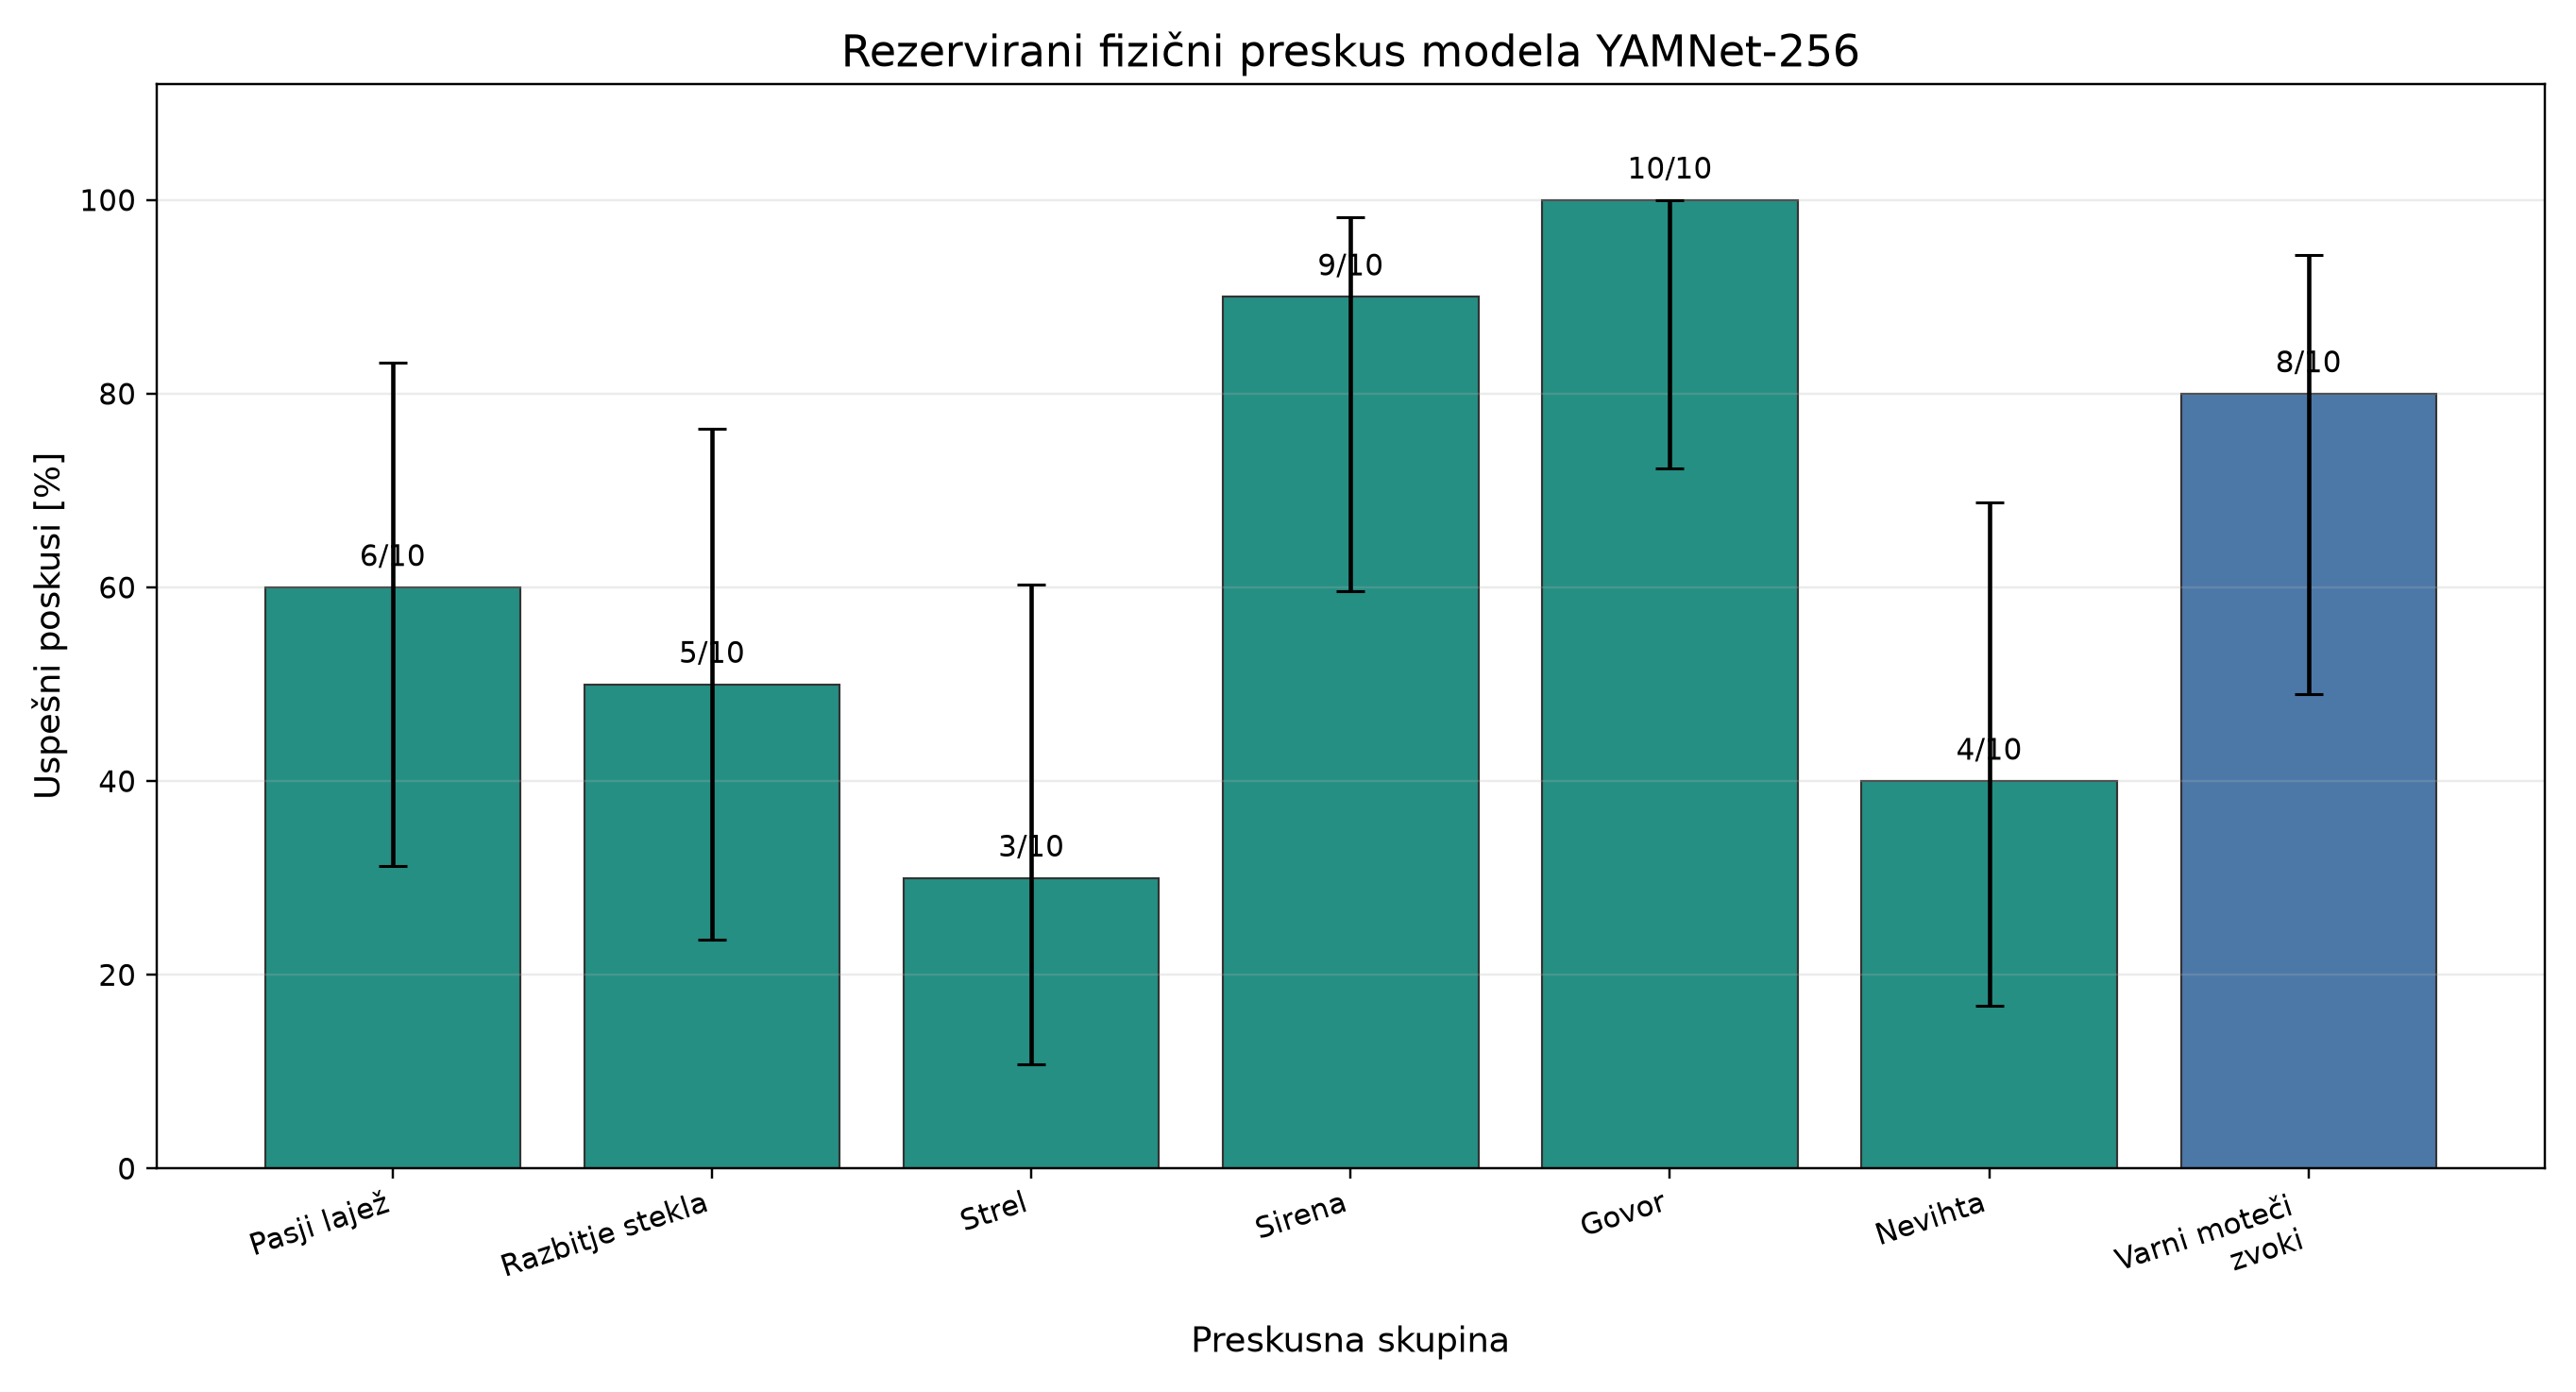
\includegraphics[width=0.94\textwidth]{../experiments/results/thesis_ch6/reserved_detection_rates_sl.png}
  \caption{Potrjene zaznave predhodne izvedbe YAMNet-256. Črte prikazujejo
  petindevetdesetodstotna Wilsonova območja zaupanja. Pri zahtevnih negativnih
  zvokih je prikazan delež varnih izidov.}
  \label{fig:rezervirani-delezi}
\end{figure}
\clearpage

\section{Lažni alarmi predhodne izvedbe}

Govor je bil v model vključen kot varen razred, da običajnega človeškega glasu
ne bi zamenjeval z nevarnostjo. Kljub pravilno zaznanemu govoru v vseh desetih
pozitivnih poskusih je v enem od njih za kratek čas nastal tudi potrjen
nevarnostni izhod. Opaženi delež takšnih lažnih alarmov je bil zato 1 od 10.

Med desetimi zahtevnimi negativnimi zvoki sta dva sprožila potrjen nevarnostni
alarm, osem pa jih je imelo varen izid. Šest od desetih primerov ni preseglo
praga vhodne aktivnosti. To ni napaka prenosa zvoka, temveč odziv naprave pri
izbranem pragu: obdelava je zvok prejela, vendar ga ni obravnavala kot dovolj
izrazitega za odločanje. Zaradi samo desetih negativnih primerov rezultat
\SI{20}{\percent} lažnih nevarnostnih alarmov opisuje ta preskus in ni ocena
pričakovane pogostosti lažnih alarmov pri dolgotrajni uporabi.

\section{Sprejemni preskus končne naprave}
\label{sec:rezultati-sprejemni}

Končna naprava z modelom YAMNet-1024 je uspešno opravila 18 od 21 poskusov
nadzorovanega sprejemnega preskusa, kar pomeni \SI{85.7}{\percent}. Pri
nominalni ravni je bilo uspešnih 8 od 9 poskusov oziroma
\SI{88.9}{\percent}. Med 18 pozitivnimi poskusi je bil pričakovani razred
potrjen v 15 primerih, vsi trije varni negativni zvoki pa so bili obravnavani
brez potrjenega nevarnostnega alarma.

\begin{table}[H]
  \centering
  \caption{Uspešnost sprejemnega preskusa končne naprave po razredih.}
  \label{tab:sprejemni-rezultati-razredi}
  \begin{tabular}{lrrrr}
    \toprule
    Razred & Nominalno & \SI{-6}{\decibel} & \SI{-12}{\decibel} & Skupaj \\
    \midrule
    Pasji lajež       & 1 od 1 & 1 od 1 & 1 od 1 & 3 od 3 \\
    Razbitje stekla   & 1 od 1 & 1 od 1 & 0 od 1 & 2 od 3 \\
    Strel             & 1 od 1 & 1 od 1 & 1 od 1 & 3 od 3 \\
    Sirena            & 1 od 1 & 1 od 1 & 1 od 1 & 3 od 3 \\
    Govor             & 1 od 1 & 1 od 1 & 0 od 1 & 2 od 3 \\
    Nevihta           & 0 od 1 & 1 od 1 & 1 od 1 & 2 od 3 \\
    \midrule
    Pozitivni zvoki   & 5 od 6 & 6 od 6 & 4 od 6 & 15 od 18 \\
    Varni zvoki       & 3 od 3 & --     & --     & 3 od 3 \\
    \bottomrule
  \end{tabular}
\end{table}

Pasji lajež, strel in sirena so bili uspešno potrjeni pri vseh treh ravneh.
Razbitje stekla in govor pri ravni \SI{-12}{\decibel} nista presegla praga
vhodne aktivnosti. Pri nevihti na nominalni ravni je bil pričakovani razred v
več aktivnih blokih na prvem mestu, vendar ni bil v dveh zaporednih blokih
dovolj močan za potrditev. To je edini neuspeh, pri katerem je dogodek prestal
energijski prag, ustavil pa ga je odločitveni pogoj.

\begin{figure}[!ht]
  \centering
  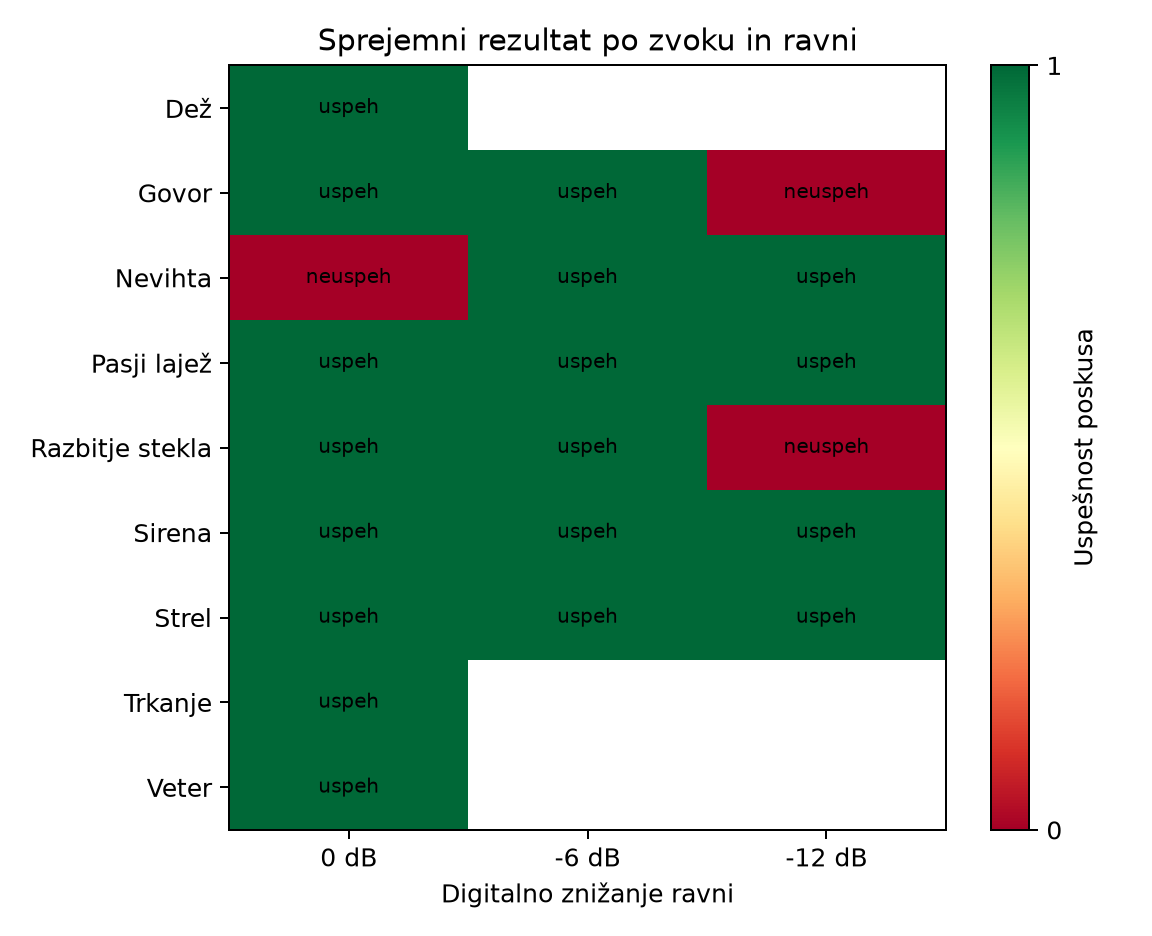
\includegraphics[width=0.94\textwidth]{../experiments/results/hazard6_v3_acceptance/trial_matrix.png}
\caption{Izid posameznih poskusov sprejemnega preskusa končne naprave.}
  \label{fig:sprejemni-matrika}
\end{figure}

\begin{figure}[!ht]
  \centering
  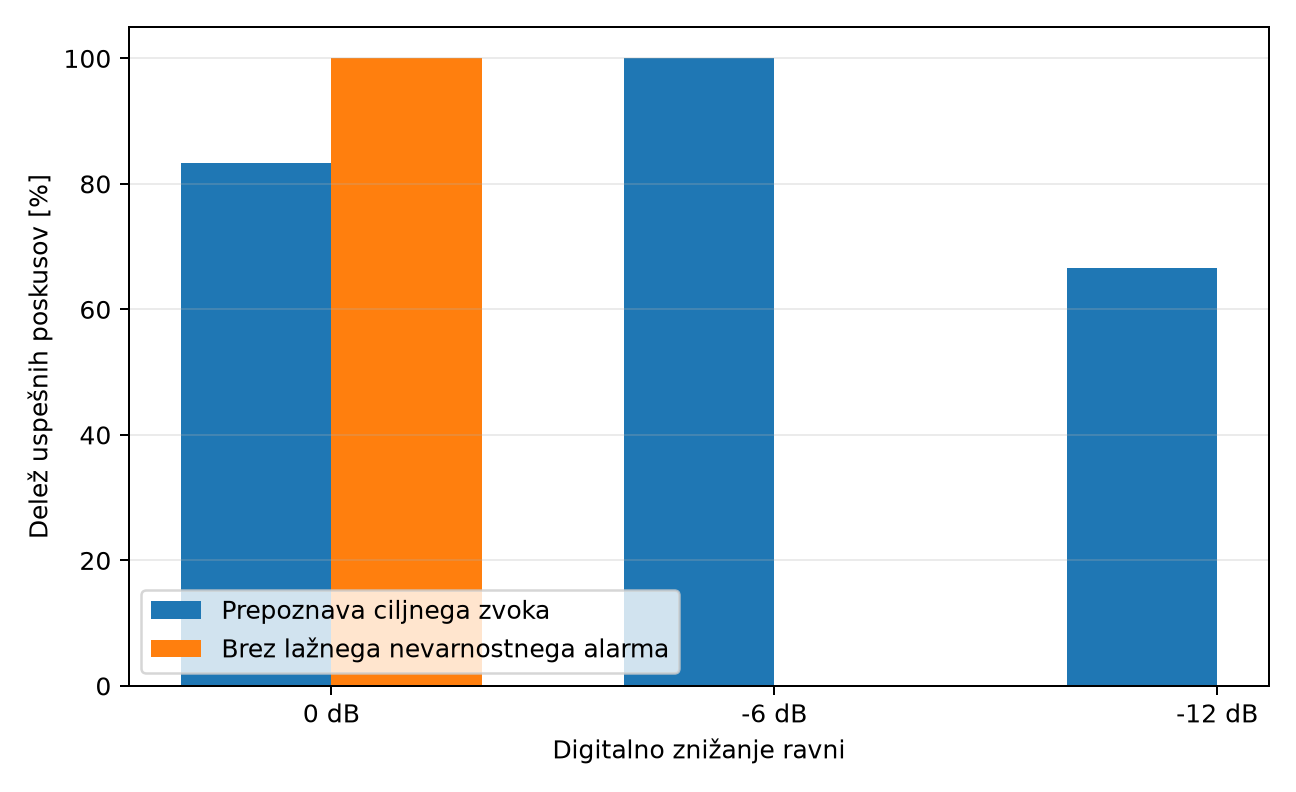
\includegraphics[width=0.82\textwidth]{../experiments/results/hazard6_v3_acceptance/pass_rate_by_level.png}
  \caption{Opaženi delež uspešnih poskusov pri posamezni ravni predvajanja.}
  \label{fig:sprejemni-ravni}
\end{figure}
\clearpage

Pri pozitivnih poskusih je bil delež uspeha pri nominalni ravni
\SI{83.3}{\percent}, pri \SI{-6}{\decibel} \SI{100}{\percent} in pri
\SI{-12}{\decibel} \SI{66.7}{\percent}. Iz tega ne smemo sklepati, da
utišanje izboljša zaznavanje. Vsaka kombinacija posnetka in ravni je bila
predvajana samo enkrat, rezultat kratkega dogodka pa je odvisen tudi od njegove
poravnave z mejo obdelovalnega bloka ter trenutnega šuma v prostoru. Preskus zato
predvsem potrjuje, da celotna končna izvedba deluje na izbranih in predhodno
pregledanih primerih. Ne predstavlja neodvisne ocene posploševanja modela na
nove zvočne vire.

\section{Neodvisni končni fizični preizkus}
\label{sec:rezultati-koncni}

V neodvisnem končnem fizičnem preizkusu je sistem pričakovani razred vsaj
enkrat potrdil v 57 od 60 poskusov. Opaženi delež je
\SI{95.0}{\percent}, Wilsonovo petindevetdesetodstotno območje zaupanja pa od
\SI{86.3}{\percent} do \SI{98.3}{\percent}. Štirje nevarnostni razredi skupaj
so bili potrjeni v 39 od 40 poskusov oziroma \SI{97.5}{\percent}.

\begin{table}[htbp]
  \centering
  \caption{Rezultati neodvisnega končnega fizičnega preizkusa.}
  \label{tab:koncni-rezultati}
  \small
  \begin{tabular}{lrrr}
    \toprule
    Razred & Uspešni poskusi & Delež & \shortstack{Wilsonovo območje\\zaupanja} \\
    \midrule
    Pasji lajež       & 10 od 10 & \SI{100}{\percent} & 72,2--100 \\
    Razbitje stekla   & 10 od 10 & \SI{100}{\percent} & 72,2--100 \\
    Strel             & 10 od 10 & \SI{100}{\percent} & 72,2--100 \\
    Ostalo            & 9 od 10  & \SI{90}{\percent}  & 59,6--98,2 \\
    Sirena            & 9 od 10  & \SI{90}{\percent}  & 59,6--98,2 \\
    Govor             & 9 od 10  & \SI{90}{\percent}  & 59,6--98,2 \\
    \midrule
    Skupaj            & 57 od 60 & \SI{95.0}{\percent} & 86,3--98,3 \\
    \bottomrule
  \end{tabular}
\end{table}

\begin{figure}[htbp]
  \centering
  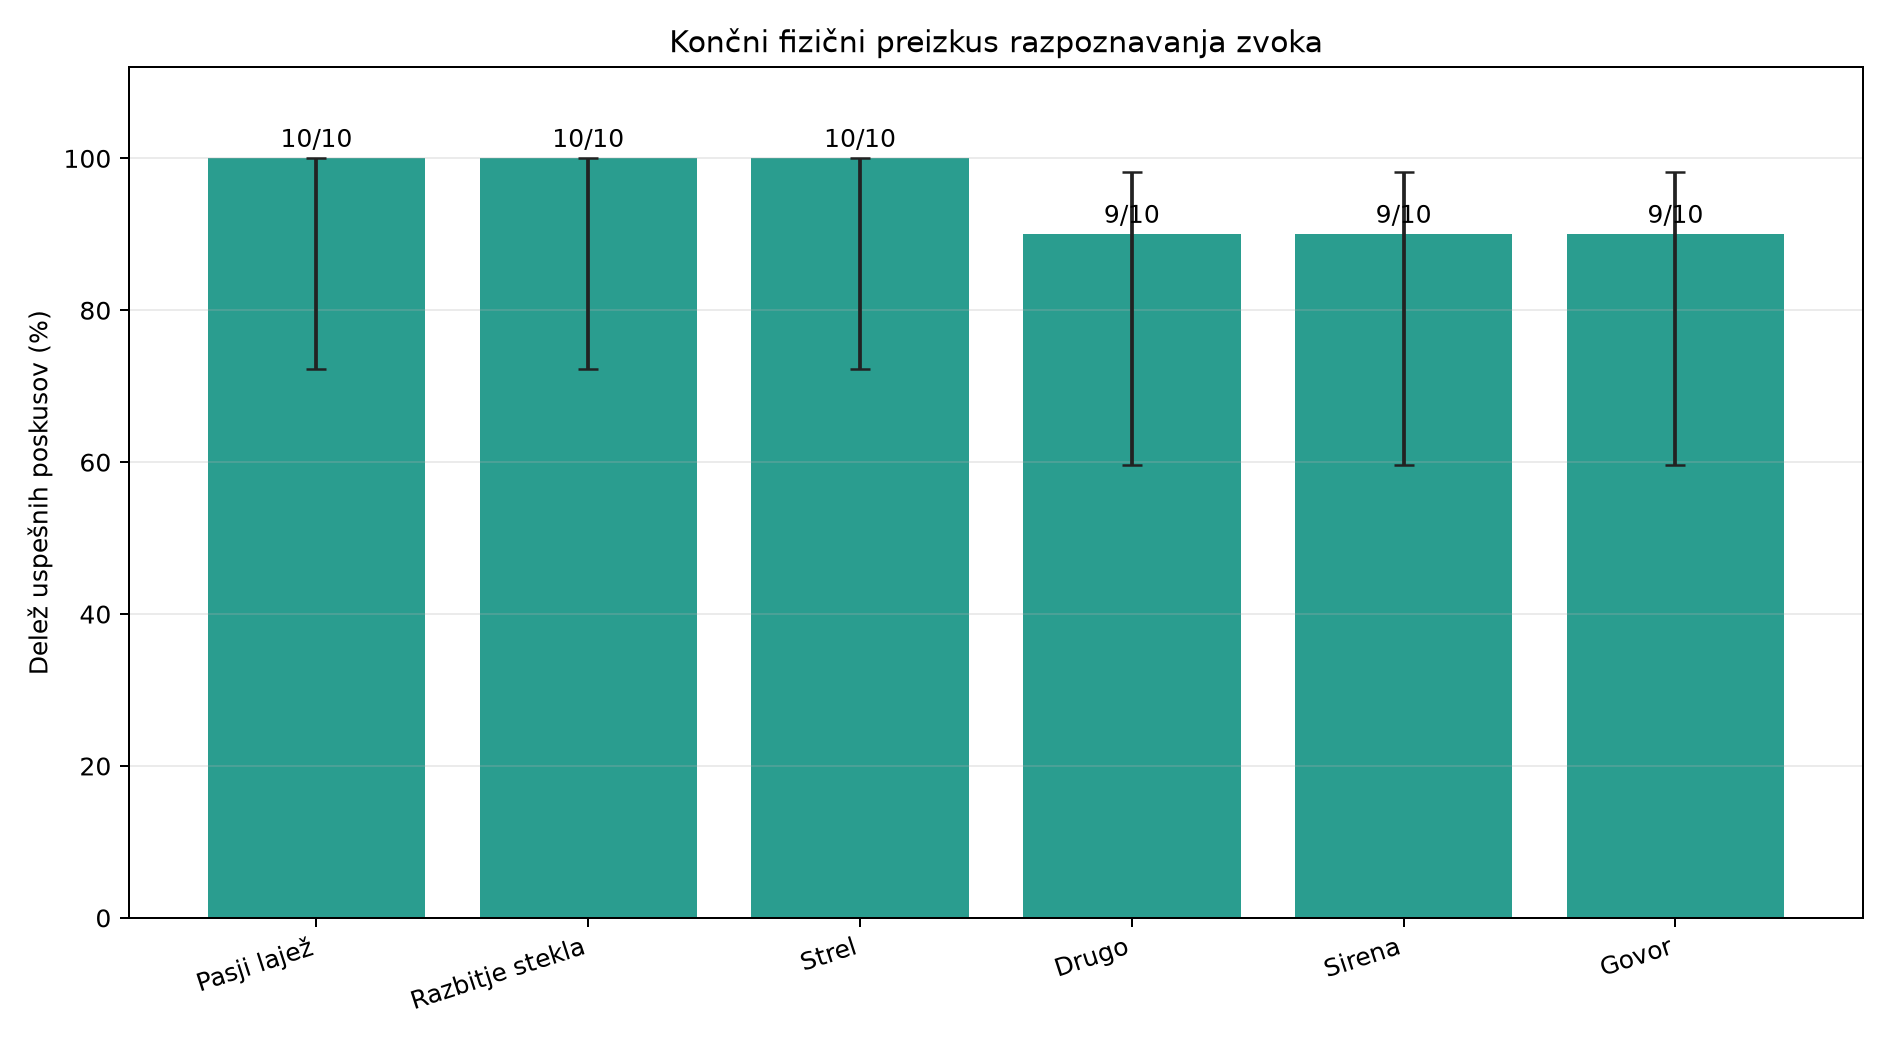
\includegraphics[width=0.96\textwidth]{../experiments/results/hazard6_final_evaluation_v4_independent/detection_rates.png}
  \caption{Delež poskusov z vsaj eno pravilno potrditvijo v neodvisnem
  končnem preizkusu. Črte prikazujejo Wilsonova petindevetdesetodstotna
  območja zaupanja.}
  \label{fig:koncni-delezi}
\end{figure}

Primarno merilo poskus šteje kot uspešen že ob eni pravilni potrditvi. Strožje
merilo prevladujočega potrjenega izhoda se je s pričakovanim razredom ujemalo v
54 od 60 poskusov oziroma \SI{90.0}{\percent}. Razlika nastane, kadar sistem
pričakovani razred sicer potrdi, vendar je drug izhod med istim predvajanjem
potrjen v več blokih. En poskus strela je imel tako prevladujoči izhod
razbitja stekla, dva uspešna govorna poskusa pa prevladujoči izhod ostalo.

\begin{figure}[htbp]
  \centering
  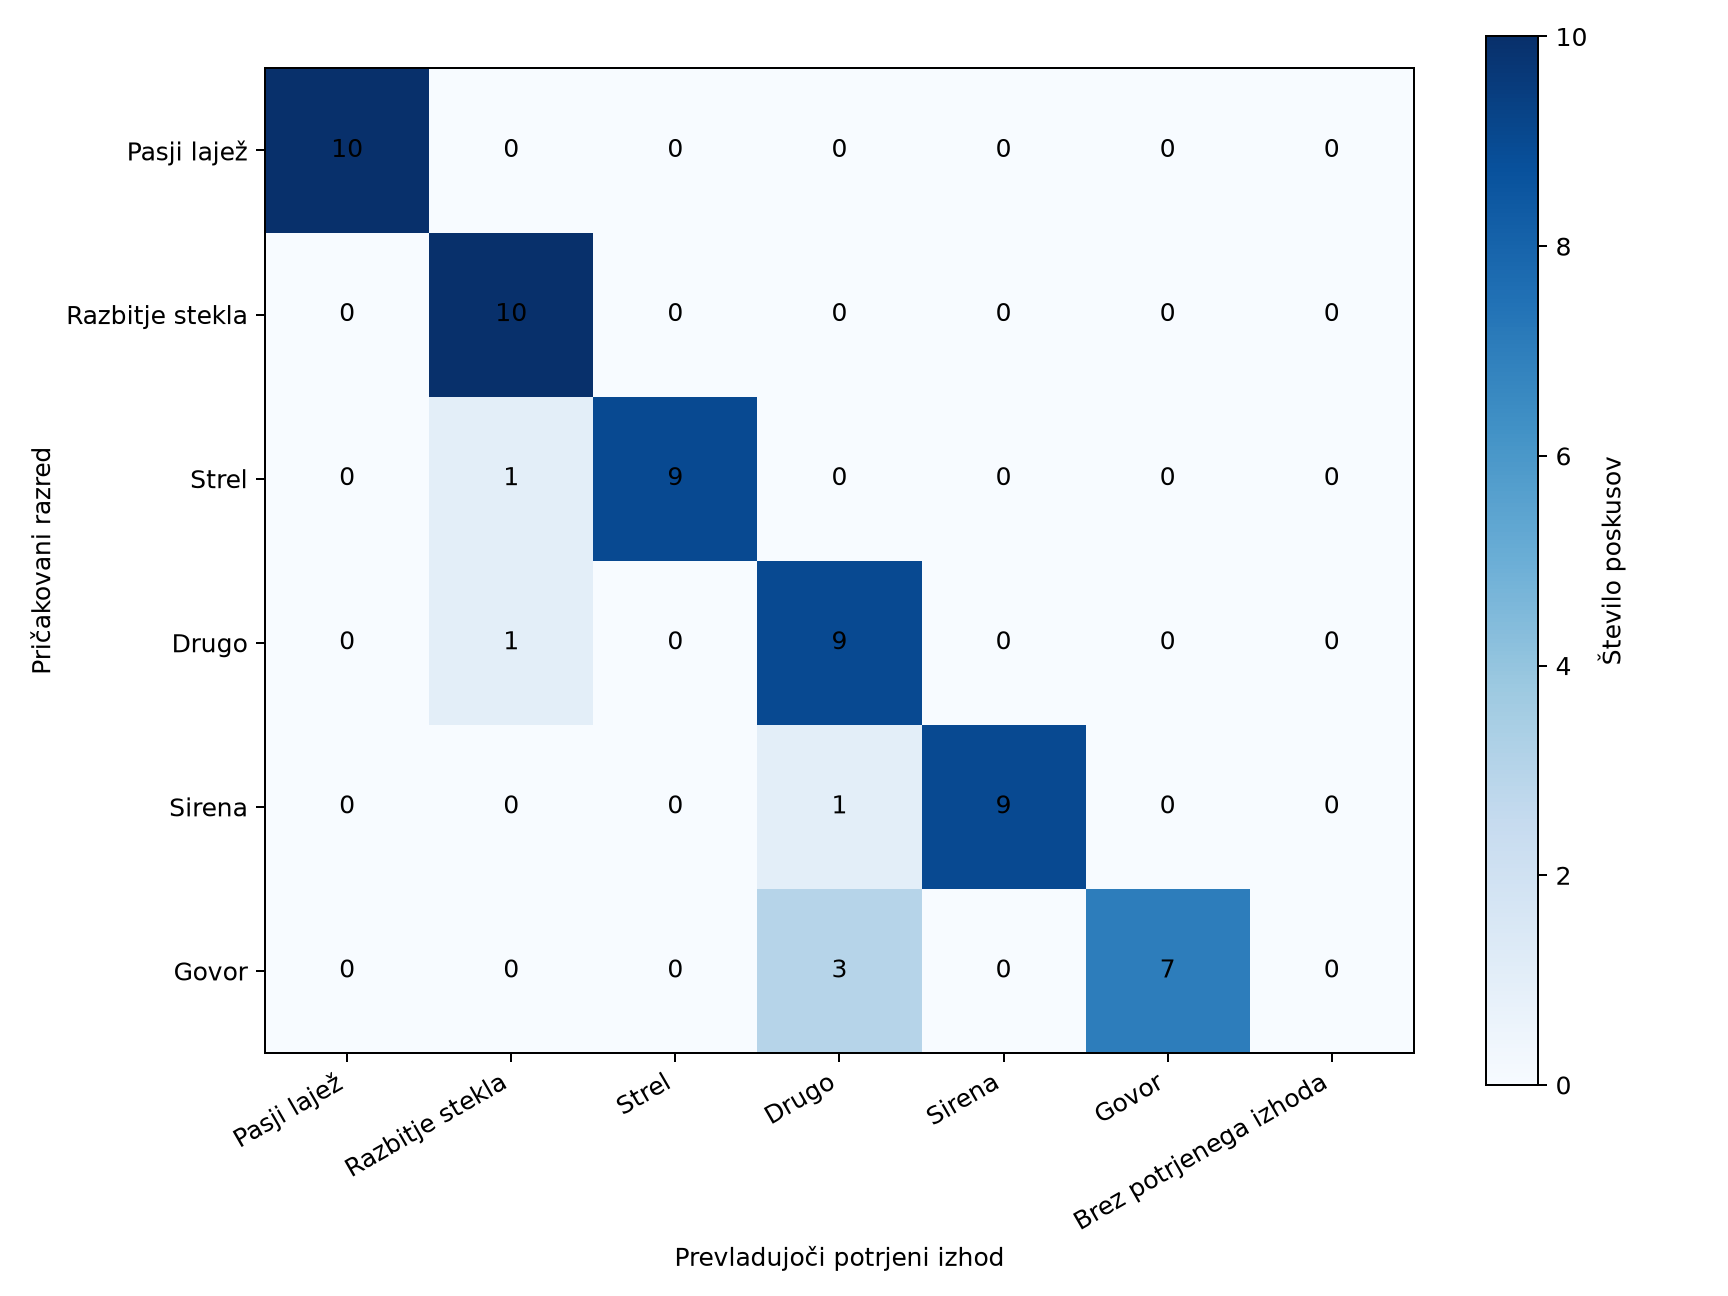
\includegraphics[width=0.88\textwidth]{../experiments/results/hazard6_final_evaluation_v4_independent/dominant_output_confusion_matrix.png}
  \caption{Matrika prevladujočih potrjenih izhodov. Primarno merilo na sliki
  \ref{fig:koncni-delezi} je drugačno, ker upošteva vsaj eno pravilno
  potrditev.}
  \label{fig:koncni-matrika}
\end{figure}

Trije neuspešni poskusi so zbrani v tabeli \ref{tab:koncni-neuspehi}. Pri
govoru je najvišja ocena pričakovanega razreda znašala 0,357 in ni dosegla
vstopnega praga 0,40. Kratek pok razreda ostalo je bil v 17 blokih potrjen
kot razbitje stekla. Pri neuspešni sireni je modelska ocena sirene dosegla
0,595, kar je ostalo pod pragom 0,65; prevladujoči potrjeni izhod je bil ostalo.

\begin{table}[htbp]
  \centering
  \caption{Neuspešni poskusi neodvisnega končnega preizkusa.}
  \label{tab:koncni-neuspehi}
  \small
  \begin{tabular}{llllr}
    \toprule
    Poskus & Pričakovano & Vrsta vira & Prevladujoči izhod & Najvišja ocena \\
    \midrule
    FE4-010 & Govor  & govor  & Ostalo            & 0,357 \\
    FE4-032 & Ostalo & pok    & Razbitje stekla   & 0,360 \\
    FE4-058 & Sirena & sirena & Ostalo            & 0,595 \\
    \bottomrule
  \end{tabular}
\end{table}

\subsection{Lažni nevarnostni alarmi}

Pri desetih govornih poskusih po začetku predvajanja ni bilo nobenega
potrjenega nevarnostnega izhoda. Pri razredu ostalo se je nevarnostni izhod vsaj
enkrat pojavil v šestih od desetih poskusov. V štirih od skupno 20 varovalnih
poskusov je ostal potrjen v več kot enem bloku. En dodaten nevarnostni izhod je bil v
celotnem zajemu govora zabeležen pred začetkom predvajanja; analiza ga je
pravilno ločila kot preneseno stanje prejšnjega poskusa.

Rezultat 9 od 10 pravilnih zaznav razreda ostalo in šest poskusov z lažnim
alarmom se ne izključujeta. V petih poskusih je sistem v delu predvajanja
pravilno potrdil ostalo, v drugem delu istega posnetka pa tudi nevarnostni
razred. Slika \ref{fig:koncni-lazni-ostalo} pokaže, da je bil najtežji pok, ki
je prevladal kot razbitje stekla. Pri aplavzu je bil strel potrjen v štirih
blokih, ploskanje, tipkovnica, alarm in trkanje pa so povzročili krajše
potrditve razbitja stekla.

\begin{figure}[htbp]
  \centering
  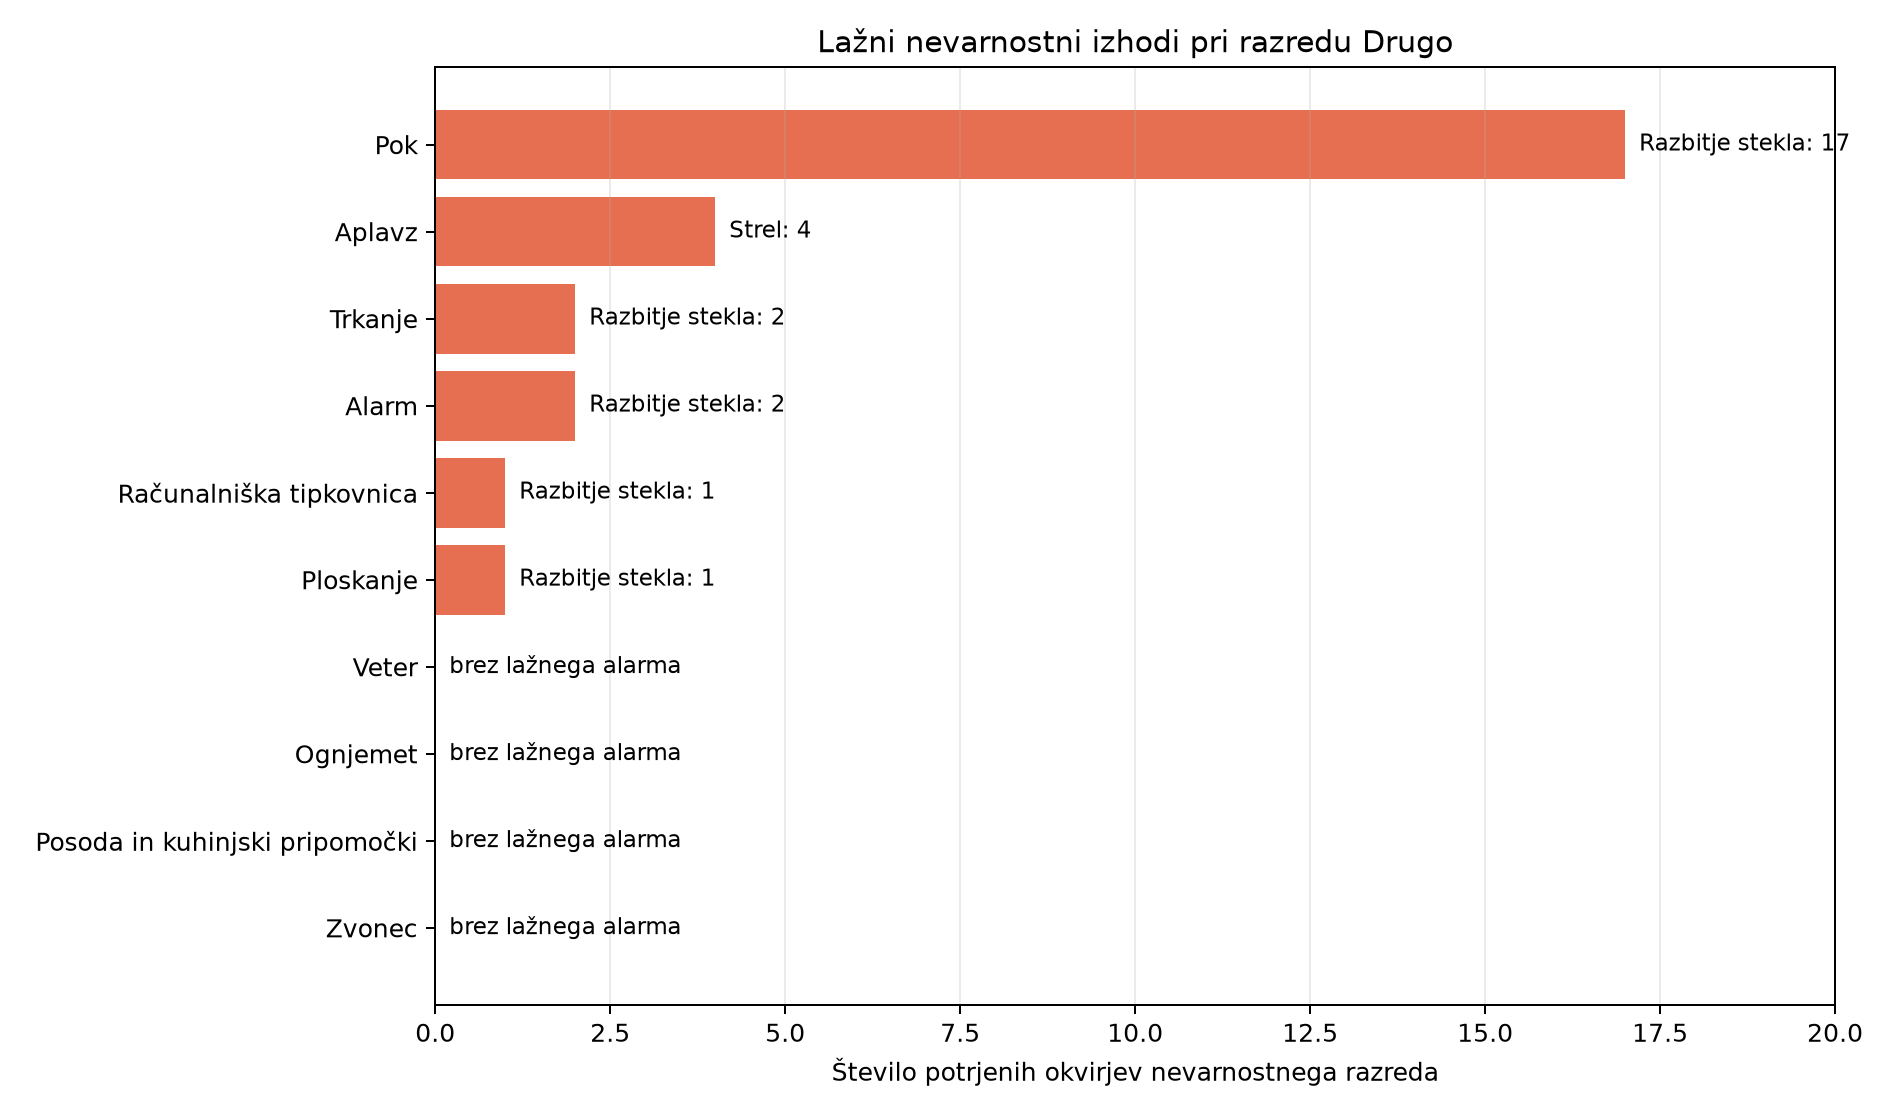
\includegraphics[width=0.96\textwidth]{../experiments/results/hazard6_final_evaluation_v4_independent/other_false_hazard_by_category.png}
  \caption{Število blokov s potrjenim nevarnostnim izhodom pri desetih vrstah
  razreda ostalo.}
  \label{fig:koncni-lazni-ostalo}
\end{figure}

\subsection{Čas do prve pravilne potrditve}

Mediana časa od začetka predvajanja do prve pravilne potrditve je bila med
\SI{1.00}{\second} za razbitje stekla in \SI{2.50}{\second} za razred ostalo.
Pri tem ne merimo samo računanja modela. Vrednost vključuje morebitno tišino
na začetku posnetka, položaj dogodka, zbiranje skoraj enosekundnega vhodnega
bloka in zahtevano število potrditvenih blokov.

\begin{figure}[htbp]
  \centering
  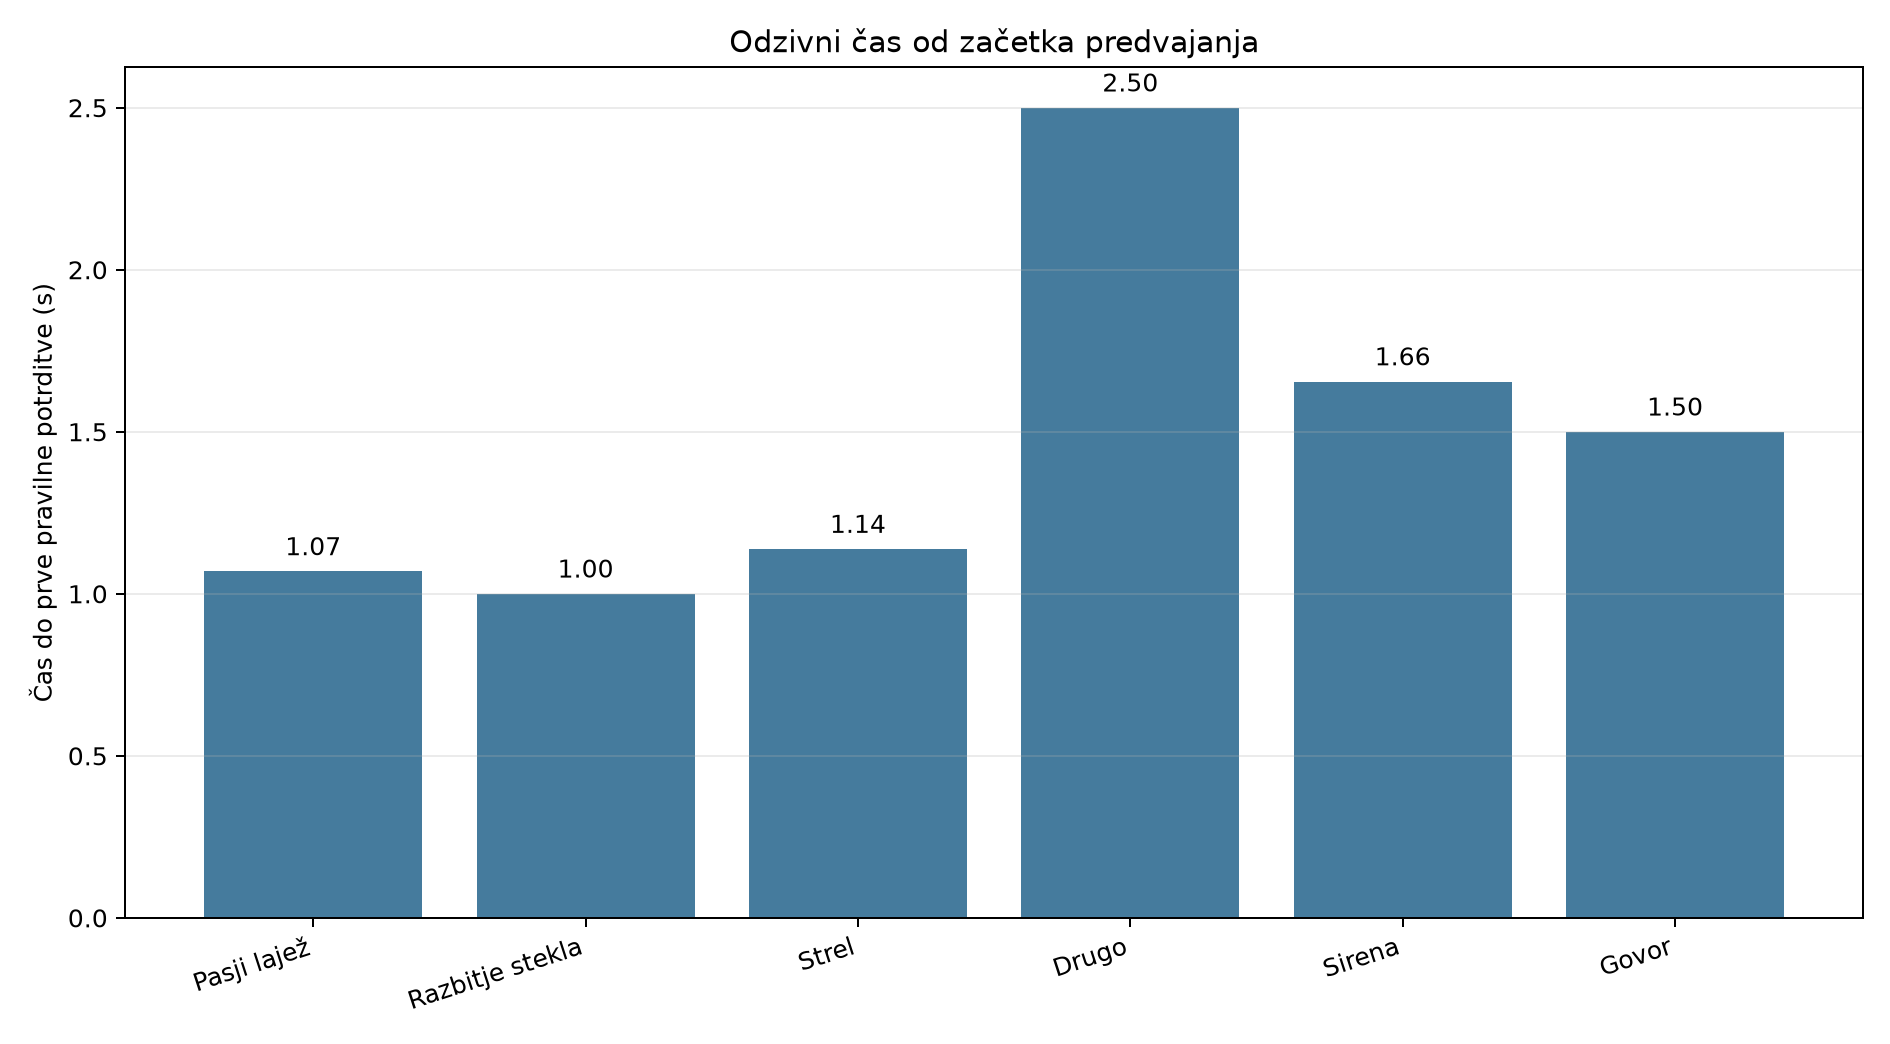
\includegraphics[width=0.94\textwidth]{../experiments/results/hazard6_final_evaluation_v4_independent/confirmation_latency.png}
  \caption{Mediana časa od začetka predvajanja do prve pravilne potrditve.}
  \label{fig:koncni-odzivni-cas}
\end{figure}

\section{Čas izvajanja}
\label{sec:rezultati-cas}

V rezerviranem preskusu izvedbe YAMNet-256 je bilo zbranih 1.438 časovnih
opazovanj. Pri sprejemnem preskusu prve šestrazredne izvedbe YAMNet-1024 je
bilo 269 popolnih zapisov, neodvisni končni preizkus sedemizhodne izvedbe pa je
vseboval 1.837 popolnih časovnih zapisov. Povprečni in mediani so bili v
zadnjem preskusu enaki zaradi ločljivosti poročane telemetrije. Časi so zbrani
v tabeli \ref{tab:primerjava-casov}.

\begin{table}[H]
  \centering
  \caption{Čas obdelave enega vhodnega bloka na napravi.}
  \label{tab:primerjava-casov}
  \small
  \begin{tabular}{lrrr}
    \toprule
    Stopnja & YAMNet-256 & \shortstack{Prvi\\YAMNet-1024} & \shortstack{Končni\\YAMNet-1024} \\
    \midrule
    Predobdelava & \SI{0.69}{\milli\second} & \SI{0.71}{\milli\second} & \SI{1.43}{\milli\second} \\
    Izvajanje nevronske mreže & \SI{0.16}{\milli\second} & \SI{4.63}{\milli\second} & \SI{9.38}{\milli\second} \\
    Skupaj & \SI{0.85}{\milli\second} & \SI{5.34}{\milli\second} & \SI{10.81}{\milli\second} \\
    \bottomrule
  \end{tabular}
\end{table}

\begin{figure}[H]
  \centering
  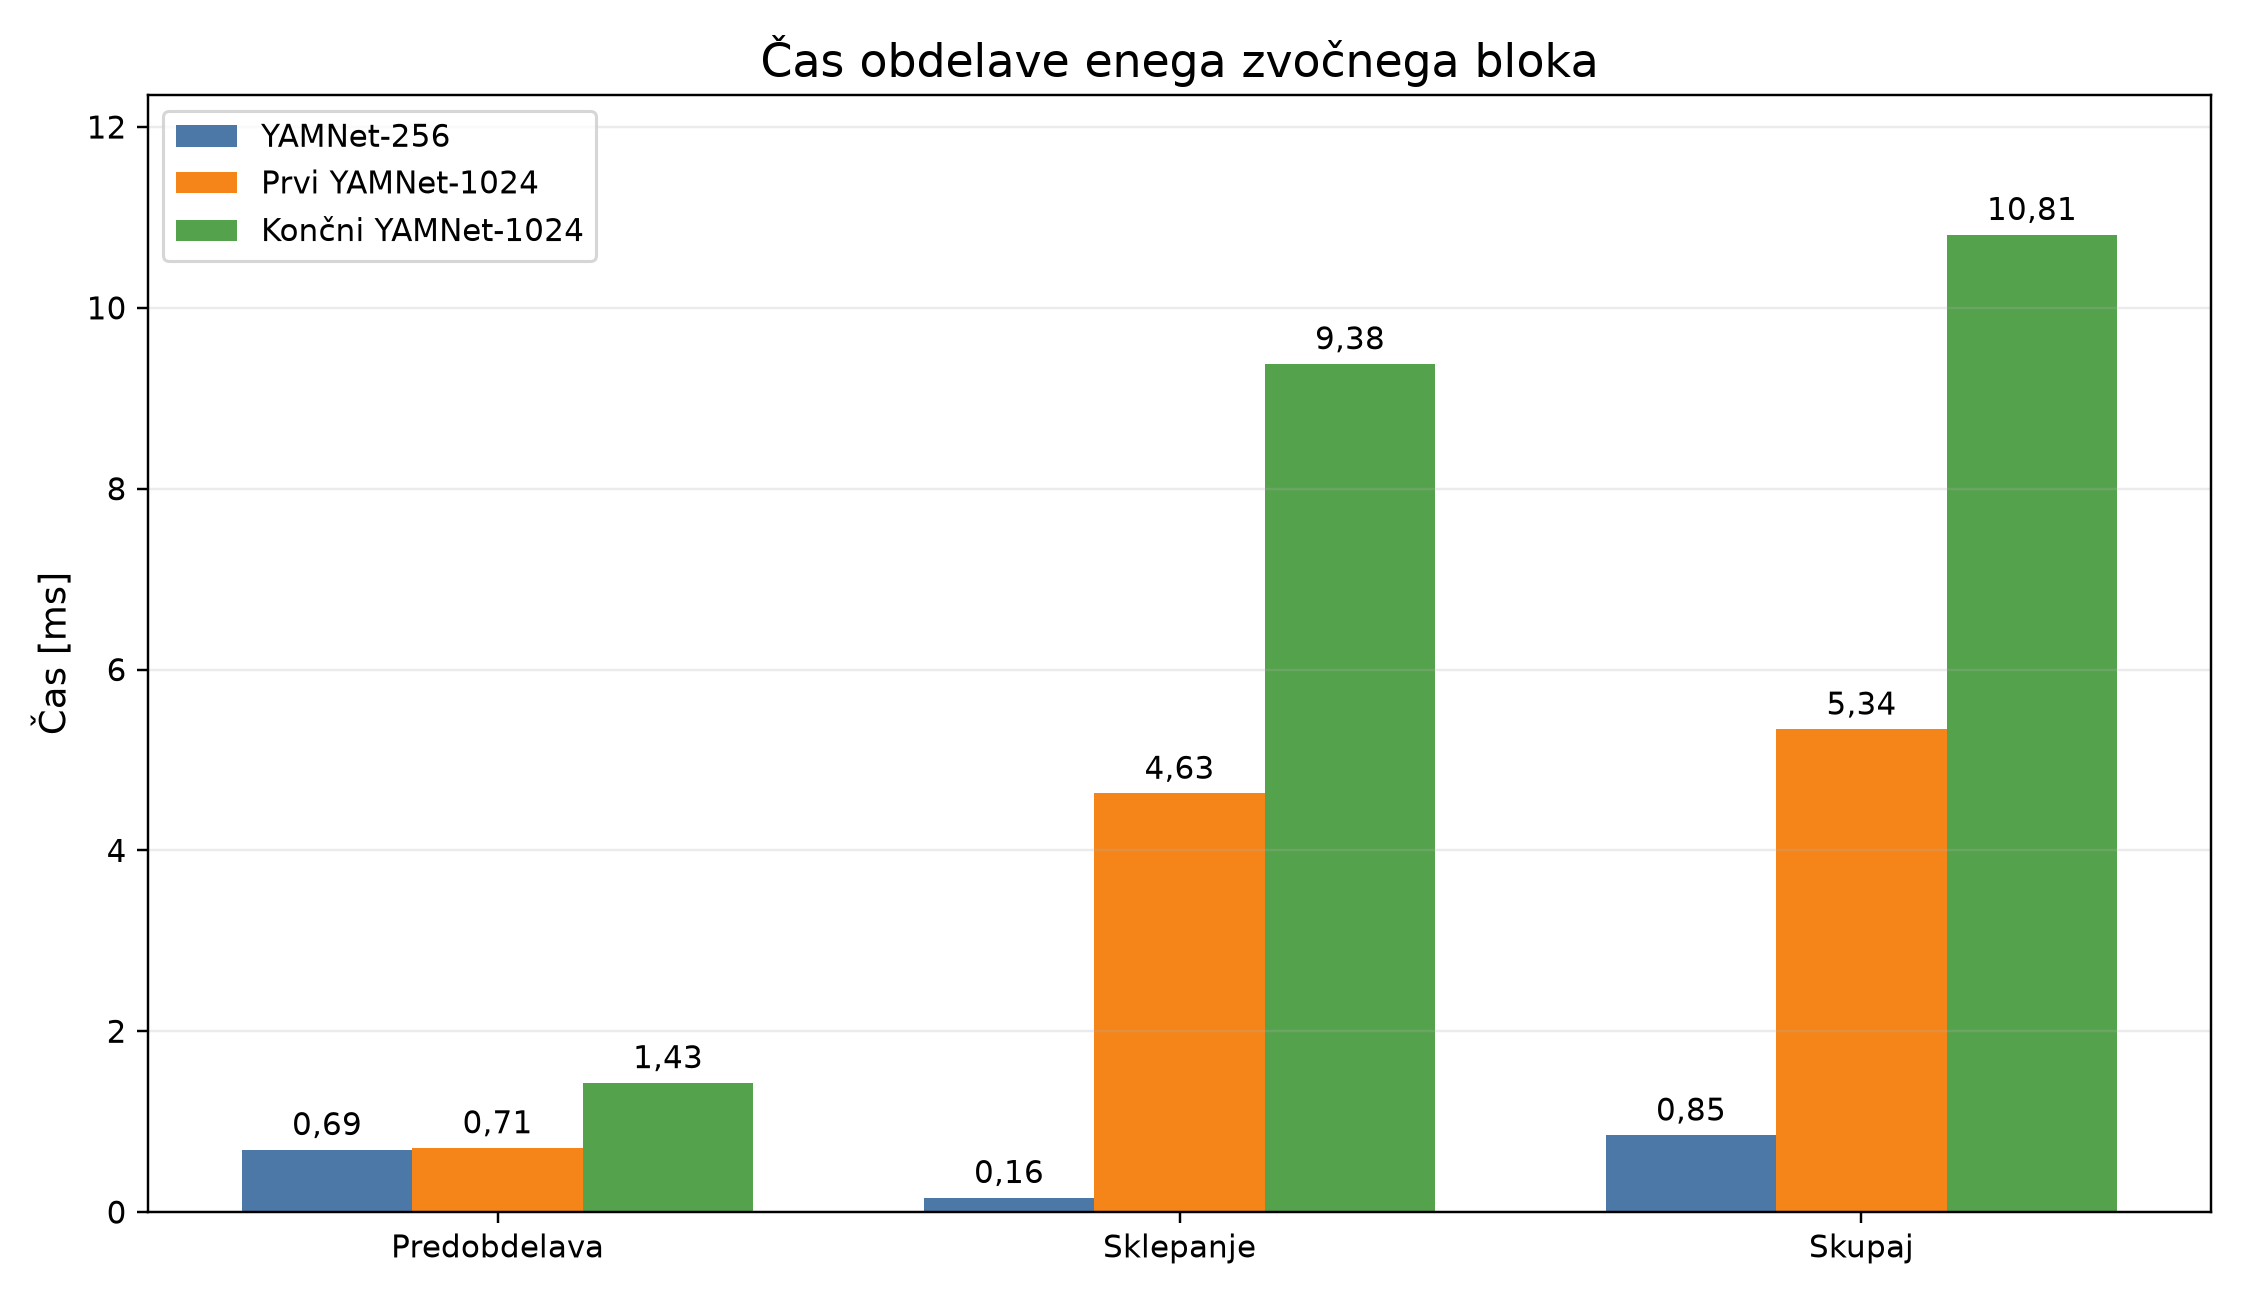
\includegraphics[width=0.88\textwidth]{../experiments/results/thesis_ch6/timing_comparison_sl.png}
  \caption{Primerjava časov obdelovalnih stopenj treh ovrednotenih izvedb.}
  \label{fig:primerjava-casov}
\end{figure}

Končna različica je zaradi večjega modela YAMNet in dodatnega izhoda
računsko zahtevnejša od začetne. Kljub temu je skupnih
\SI{10.81}{\milli\second} približno 44-krat manj od
\SI{480}{\milli\second} med začetkoma dveh zaporednih obdelav. Računska pot
zasede približno \SI{2.25}{\percent} tega intervala, zato ostane dovolj rezerve
za zajem zvoka in osveževanje zaslona.

Izvedba istega modela samo na procesorskem jedru ni bila izmerjena, zato iz teh
rezultatov ne izpeljujemo številčnega faktorja pohitritve Neural-ART. Meritev
\SI{9.38}{\milli\second} opisuje prevedeno izvedbo, v kateri je 29 od 34
izvedbenih odsekov dodeljenih pospeševalniku.

Izmerjenih \SI{10.81}{\milli\second} ni celotna zakasnitev zaznave. Naprava mora
najprej zbrati vhodni zvočni blok, odločitveni filter pa lahko zahteva še
potrditev v naslednjem bloku. Meritev zato dokazuje veliko časovno rezervo
računske poti, ne pa odziva v nekaj milisekundah od nastanka zvoka.

\section{Pomnilniški in računski odtis}
\label{sec:rezultati-pomnilnik}

Tabela \ref{tab:pomnilniski-odtis} primerja pomnilniški odtis predhodne in
končne izvedbe. Vrednosti pripadajo različnim fizičnim pomnilniškim območjem,
zato jih med seboj ne seštevamo. Stolpec izrabe prikazuje zasedenost
razpoložljivega območja pri končni izvedbi.

\begin{table}[H]
  \centering
  \caption{Primerjava pomnilniškega odtisa izvedb YAMNet-256 in YAMNet-1024.}
  \label{tab:pomnilniski-odtis}
  \small
  \begin{tabular}{>{\raggedright\arraybackslash}p{0.30\textwidth}
                  >{\centering\arraybackslash}p{0.14\textwidth}
                  >{\centering\arraybackslash}p{0.14\textwidth}
                  >{\centering\arraybackslash}p{0.14\textwidth}
                  >{\centering\arraybackslash}p{0.10\textwidth}}
    \toprule
    Pomnilniško območje & YAMNet-256 & YAMNet-1024 & \shortstack{Na\\voljo} & Izraba \\
    \midrule
    Notranji pomnilnik aplikacije
      & 582,2 KiB & 595,1 KiB & 1.023 KiB & \SI{58.2}{\percent} \\
    Aktivacije nevronskega pospeševalnika
      & 144,0 KiB & 240,0 KiB & 448 KiB & \SI{53.6}{\percent} \\
    Zaslonska medpomnilnika v zunanjem pomnilniku
      & 1.500,0 KiB & 1.500,0 KiB & 16.384 KiB & \SI{9.2}{\percent} \\
    Podpisana programska slika
      & 229,9 KiB & 244,3 KiB & 512 KiB & \SI{47.7}{\percent} \\
    Prevedene uteži v zunanjem bliskovnem pomnilniku
      & 145,2 KiB & 3.203,7 KiB & 64.512 KiB & \SI{5.0}{\percent} \\
    \bottomrule
  \end{tabular}
\end{table}

Največja sprememba je nastala pri utežeh, ki so se povečale približno
22-krat, in pri aktivacijskem pomnilniku, ki se je povečal za približno
1,67-krat. Velikost povezane aplikacije v notranjem pomnilniku se je povečala
le za približno \SI{0.7}{\percent}, podpisana programska slika pa za približno
\SI{2.5}{\percent}. Zaslonska medpomnilnika sta ostala nespremenjena. Večji
model se zato ni približal omejitvi zunanjega bliskovnega pomnilnika, prav tako
pa je v območju za aktivacije ostalo približno \SI{46}{\percent} prostora.

Datoteka izvedljive in povezovalne oblike vsebuje tudi simbole in druge podatke
za razhroščevanje, zato njena velikost ni enaka velikosti programske slike na
napravi. Dejanska podpisana binarna slika končne aplikacije ima 250.176 bajtov,
povezovalnik pa za izvajanje aplikacije navaja 609.372 bajtov notranjega
pomnilnika.

Poročilo prevajalnika modela za en prehod navaja 71.146.316 operacij množenja
in seštevanja. Izvajalni načrt je razdeljen na 34 odsekov: 29 jih izvede
nevronski pospeševalnik, pet pa procesorsko jedro. Programsko izvedeni odseki
so povezani predvsem s pretvorbami na mejah modela in z njegovo zaključno
plastjo. Izraz \emph{odsek} tu ne pomeni učnega prehoda, temveč del že
naučenega omrežja, ki ga je prevajalnik dodelil določeni strojni enoti. Večino
računsko zahtevnih plasti tako izvede Neural-ART, kar omogoča izmerjeni čas
\SI{9.38}{\milli\second} kljub več kot 71 milijonom operacij.

\section{Povzetek rezultatov}

Rezultati kažejo potek od odkritih pomanjkljivosti do izboljšane končne
izvedbe. Rezervirani fizični preskus YAMNet-256 je dosegel 37 potrjenih pravilnih
zaznav v 60 pozitivnih poskusih in je pokazal predvsem šibkost pri strelu,
razbitju stekla in nevihti. Na podlagi teh ugotovitev so bili izboljšani izbor
dogodkov, povečanje učnih podatkov, prehod na YAMNet-1024 in odločitveno pravilo
za nevihto.

Končni razvojni model YAMNet-1024 je pravilno razvrstil 333 od 413 razvojnih
posnetkov. Neodvisni končni fizični preizkus je nato dosegel vsaj eno pravilno
potrditev v 57 od 60 poskusov, strožje merilo prevladujočega izhoda pa v 54 od
60 poskusov. Pri štirih nevarnostnih razredih je bilo pravilnih 39 od 40
poskusov. Glavna preostala pomanjkljivost je zavračanje nekaterih drugih
kratkih in izrazitih zvokov: nevarnostni izhod se je pojavil pri šestih od
desetih poskusov razreda ostalo, pri štirih pa je ostal potrjen v več kot enem
bloku.

Prehod na večji model in razširjeni razred ostalo sta povečala čas izvajanja in
pomnilniški odtis, vendar je končna izvedba ostala znotraj vseh pomnilniških
območij. Skupna obdelava enega bloka traja \SI{10.81}{\milli\second}, zato ima
sistem pri novem bloku vsakih \SI{480}{\milli\second} veliko časovno rezervo.
Rezultati potrjujejo delovanje celotne poti na izbrani postavitvi, ne dokazujejo
pa varnostne zanesljivosti v vseh prostorih in za vse možne zvočne vire.

\chapter{Razprava in sklepne ugotovitve}
\label{ch:razprava-sklep}

\section{Odgovori na raziskovalna vprašanja}

Na prvo raziskovalno vprašanje lahko odgovorimo pritrdilno. Kvantizirani model
YAMNet-1024 se na mikrokrmilniku STM32N6 izvaja sproti. Predobdelava enega
bloka traja povprečno \SI{1.43}{\milli\second}, izvajanje nevronske mreže
\SI{9.38}{\milli\second}, skupaj pa \SI{10.81}{\milli\second}. Nov blok se
pripravi vsakih \SI{480}{\milli\second}, zato računanje porabi približno
\SI{2.25}{\percent} tega intervala. Tudi aplikacija, aktivacije, uteži in dva
zaslonska medpomnilnika ostanejo znotraj svojih pomnilniških območij. To
potrjuje tehnično izvedljivost celotne lokalne poti, ne pomeni pa, da je čas od
nastanka zvoka do opozorila samo \SI{10.81}{\milli\second}, saj mora sistem
najprej zbrati vhodni blok in po potrebi potrditi več zaporednih odločitev.

Na drugo vprašanje odgovarja neodvisni končni fizični preizkus. Sistem je
pričakovani razred vsaj enkrat potrdil v 57 od 60 poskusov oziroma v
\SI{95.0}{\percent} poskusov. Pri štirih nevarnostnih razredih je bil uspešen
v 39 od 40 poskusov. Strožje merilo prevladujočega izhoda je bilo pravilno v
54 od 60 poskusov. Govor ni sprožil nobenega nevarnostnega alarma, pri razredu
ostalo pa se je nevarnostni izhod pojavil v šestih od desetih poskusov. Sistem
je torej v preskusni postavitvi dobro zaznaval ciljne dogodke, zavračanje
nekaterih kratkih vsakdanjih zvokov pa ostaja njegova glavna slabost.

Tretje vprašanje nima enega samega odgovora za vse razrede. Pasji lajež,
razbitje stekla in strel so bili v končnem preizkusu potrjeni v vseh desetih
poskusih. Sirena, govor in ostalo so dosegli devet pravilnih potrditev od
desetih. Rezultati neuspešnih poskusov kažejo različne vzroke: ocena govora in
sirene je ostala pod razrednim pragom, kratek pok pa je bil podoben razbitju
stekla. Na delovanje zato vplivajo kakovost in glasnost vira, položaj dogodka v
skoraj enosekundnem vhodnem bloku, podobnost med razredi ter izbrani pragovi in časovna
pravila.

\section{Razprava o uporabnosti rezultatov}

Prototip je namenjen pretvarjanju izbranih nevarnih zvokov v vidno opozorilo
za gluhe in naglušne uporabnike. Njegova praktična prednost je samostojno
delovanje: mikrofon, predobdelava, model, odločanje in prikaz so na isti
napravi. Internetna povezava, oddaljeni strežnik in uporabniški račun niso
potrebni. Običajna programska oprema surovega zvoka ne shranjuje, začasni
vzorci pa se po sprotni obdelavi prepišejo. To zmanjša izpostavljenost zvoka iz
domačega okolja in hkrati omogoča delovanje tudi ob izpadu omrežja.

Zaslon jasno razlikuje med čakanjem, nezanesljivo napovedjo, običajnim zvokom
in potrjenim nevarnostnim dogodkom. Takšna izvedba je primerna kot raziskovalni
prototip in kot osnova za nadaljnji razvoj namenskega opozorilnega pripomočka.
Ni pa nadomestilo za certificiran požarni, protivlomni ali medicinski sistem.
Preizkus je obsegal nadzorovano predvajanje v enem prostoru, zato iz rezultata
ne moremo sklepati, da bo naprava enako zanesljiva pri vseh resničnih zvokih,
razdaljah in okoljih.

\section{Omejitve projekta}

V vsakem sistemskem razredu je bilo deset preskusnih posnetkov, zato so
razredna območja zaupanja široka. Zvoki so bili predvajani prek enega zvočnika
na razdalji \SI{30}{\centi\meter} v enem prostoru. Tak postopek zagotavlja
ponovljivost, ne zajame pa odmeva, oddaljenosti, prekrivanja več zvokov in
različnih mikrofonov pri vsakdanji uporabi. Uporabljeni posnetki so bili novi
glede na učenje in izbiro pragov, vendar še vedno izvirajo iz javnih zbirk in
ne iz daljšega terenskega snemanja ciljnega okolja.

Sistem pozna omejen nabor nevarnosti. Posebej zahtevni so kratki dogodki, ki
so si spektralno podobni. Razred ostalo je raznolik in ga 630 učnih virov ne
more izčrpno opisati; zato so pok, aplavz in nekateri gospodinjski zvoki še
vedno povzročili lažne nevarnostne izhode. Izmerjeni čas temelji na notranji
telemetriji, ne na zunanjem električnem signalu, poraba energije pa ni bila
izmerjena. Prav tako uporabniška študija z gluhimi ali naglušnimi osebami ni
bila izvedena. Namen za ciljno skupino je zato zasnovna motivacija, ne dokaz
klinične ali vsakdanje uporabnosti.

\section{Možnosti nadaljnjega dela}

Najpomembnejši naslednji korak je razširitev razreda ostalo z lokalnimi
gospodinjskimi zvoki ter s težkimi negativnimi primeri, pri katerih trenutni
sistem napove nevarnost. Temu naj sledi novo učenje in popolnoma ločen končni
preskus. Smiselni so preskusi na več razdaljah, v več prostorih, ob hrupu in ob
hkratnem pojavu govora ter nevarnostnega dogodka. Lasten uravnotežen nabor bi
bolje opisal pričakovano okolje kot samo javni posnetki.

Celotno zakasnitev bi bilo mogoče natančneje izmeriti z zunanjim signalom in
osciloskopom, porabo pa z merilnikom energije. Za uporabniški del bi bilo treba
skupaj z gluhimi in naglušnimi osebami preveriti razumljivost opozoril,
velikost besedila, barve ter morebitno dodajanje vibracijskega ali svetlobnega
izhoda. Morebitno razširjanje nabora nevarnosti naj temelji na dovolj kakovostnih
učnih podatkih in ločenem vrednotenju, ne le na dodajanju novih oznak.

\section{Sklepne ugotovitve}

V diplomskem delu je bil razvit samostojen sistem za zaznavanje nevarnih
zvočnih dogodkov na razvojni plošči STM32N6570-DK. Vgrajeni mikrofon
neprekinjeno zajema zvok, lastna predobdelava pripravi strnjeni spektrogram,
kvantizirani model YAMNet-1024 se izvaja z nevronskim
pospeševalnikom Neural-ART, odločitveni filter pa rezultat pretvori v stabilno
vidno opozorilo. Celotna obdelava poteka lokalno, brez dostopa do računalniškega
oblaka in brez trajnega shranjevanja surovega zvoka v običajnem delovanju.

Razvoj je pokazal, da pri vgrajenem razpoznavanju ni dovolj samo namestiti
prednaučenega modela. Za kratke dogodke so bili potrebni namensko izrezovanje,
povečanje podatkov, razred ostalo, razredni pragovi in časovno filtriranje.
Končna različica je v neodvisnem fizičnem preizkusu pravilno potrdila 57 od 60
poskusov, pri nevarnostnih razredih pa 39 od 40. Obdelava enega bloka je
trajala \SI{10.81}{\milli\second} in je ostala znotraj razpoložljivega
pomnilnika. Preostali lažni alarmi pri razredu ostalo jasno določajo naslednjo
razvojno nalogo. Glavni rezultat dela je zato delujoč in merljivo dovolj hiter
lokalni prototip ter sledljiv postopek, ki njegove prednosti loči od njegovih
še odprtih omejitev.


\begingroup
\sloppy
\printbibliography[heading=bibintoc]
\endgroup

\appendix
\chapter{Sledljivost programske opreme in rezultatov}
\label{app:sledljivost}

Končna evalvacija ima identifikator
\texttt{STM32N6-HAZARD6-FINAL-003}, poskus pa oznako \texttt{FE4-A01}.
Manifest ima naslednjo kontrolno vsoto
SHA-256:
\begin{center}
  \small\texttt{0355fca0f9a3d26be1e41b4fd9896f7}\newline
  \texttt{fb7c9f567557a7dde23826dbb36c1342b}.
\end{center}

Glavni rezultati in grafi so shranjeni v naslednjih imenikih:
\begin{itemize}
  \item \path{experiments/results/hazard6_final_evaluation_v4_independent},
  \item \path{experiments/results/deployment_footprint}.
\end{itemize}
Fotografije fizične izvedbe skupaj s kontrolnimi vsotami izvirnikov so
shranjene v imeniku \path{Doc/thesis_photos}.

Postopek priprave kratkotrajnih dogodkov je v programu
\path{ml/prepare_transient_event_windows.py}, povečanje učnega nabora pa v
\path{ml/prepare_patch_balanced_augmentation.py}. Končna učna nastavitev je v
datoteki \path{ml/configs/hazard5v5_other_yamnet1024_tqe.yaml}, zagon učenja pa
je dokumentiran v programu \path{ml/train_hazard5v5_other_yamnet1024.ps1}.
Datoteke z rezultati hranijo tudi razrešeno učno nastavitev, metrike po prehodih
in kontrolne vsote modelov.

Izvorna koda, analizni programi in zapisi o razvoju so v javnem repozitoriju
\url{https://github.com/aleksMuhicFri2/stm32n6-edge-audio-classifier}. Zaradi
licenčnih in velikostnih omejitev javne zbirke zvoka niso vključene v
repozitorij; manifesti hranijo izvorne oznake in kontrolne vsote uporabljenih
dražljajev.


\end{document}
